\documentclass[1p]{elsarticle_modified}
%\bibliographystyle{elsarticle-num}

%\usepackage[colorlinks]{hyperref}
%\usepackage{abbrmath_seonhwa} %\Abb, \Ascr, \Acal ,\Abf, \Afrak
\usepackage{amsfonts}
\usepackage{amssymb}
\usepackage{amsmath}
\usepackage{amsthm}
\usepackage{scalefnt}
\usepackage{amsbsy}
\usepackage{kotex}
\usepackage{caption}
\usepackage{subfig}
\usepackage{color}
\usepackage{graphicx}
\usepackage{xcolor} %% white, black, red, green, blue, cyan, magenta, yellow
\usepackage{float}
\usepackage{setspace}
\usepackage{hyperref}

\usepackage{tikz}
\usetikzlibrary{arrows}

\usepackage{multirow}
\usepackage{array} % fixed length table
\usepackage{hhline}

%%%%%%%%%%%%%%%%%%%%%
\makeatletter
\renewcommand*\env@matrix[1][\arraystretch]{%
	\edef\arraystretch{#1}%
	\hskip -\arraycolsep
	\let\@ifnextchar\new@ifnextchar
	\array{*\c@MaxMatrixCols c}}
\makeatother %https://tex.stackexchange.com/questions/14071/how-can-i-increase-the-line-spacing-in-a-matrix
%%%%%%%%%%%%%%%

\usepackage[normalem]{ulem}

\newcommand{\msout}[1]{\ifmmode\text{\sout{\ensuremath{#1}}}\else\sout{#1}\fi}
%SOURCE: \msout is \stkout macro in https://tex.stackexchange.com/questions/20609/strikeout-in-math-mode

\newcommand{\cancel}[1]{
	\ifmmode
	{\color{red}\msout{#1}}
	\else
	{\color{red}\sout{#1}}
	\fi
}

\newcommand{\add}[1]{
	{\color{blue}\uwave{#1}}
}

\newcommand{\replace}[2]{
	\ifmmode
	{\color{red}\msout{#1}}{\color{blue}\uwave{#2}}
	\else
	{\color{red}\sout{#1}}{\color{blue}\uwave{#2}}
	\fi
}

\newcommand{\Sol}{\mathcal{S}} %segment
\newcommand{\D}{D} %diagram
\newcommand{\A}{\mathcal{A}} %arc


%%%%%%%%%%%%%%%%%%%%%%%%%%%%%5 test

\def\sl{\operatorname{\textup{SL}}(2,\Cbb)}
\def\psl{\operatorname{\textup{PSL}}(2,\Cbb)}
\def\quan{\mkern 1mu \triangleright \mkern 1mu}

\theoremstyle{definition}
\newtheorem{thm}{Theorem}[section]
\newtheorem{prop}[thm]{Proposition}
\newtheorem{lem}[thm]{Lemma}
\newtheorem{ques}[thm]{Question}
\newtheorem{cor}[thm]{Corollary}
\newtheorem{defn}[thm]{Definition}
\newtheorem{exam}[thm]{Example}
\newtheorem{rmk}[thm]{Remark}
\newtheorem{alg}[thm]{Algorithm}

\newcommand{\I}{\sqrt{-1}}
\begin{document}

%\begin{frontmatter}
%
%\title{Boundary parabolic representations of knots up to 8 crossings}
%
%%% Group authors per affiliation:
%\author{Yunhi Cho} 
%\address{Department of Mathematics, University of Seoul, Seoul, Korea}
%\ead{yhcho@uos.ac.kr}
%
%
%\author{Seonhwa Kim} %\fnref{s_kim}}
%\address{Center for Geometry and Physics, Institute for Basic Science, Pohang, 37673, Korea}
%\ead{ryeona17@ibs.re.kr}
%
%\author{Hyuk Kim}
%\address{Department of Mathematical Sciences, Seoul National University, Seoul 08826, Korea}
%\ead{hyukkim@snu.ac.kr}
%
%\author{Seokbeom Yoon}
%\address{Department of Mathematical Sciences, Seoul National University, Seoul, 08826,  Korea}
%\ead{sbyoon15@snu.ac.kr}
%
%\begin{abstract}
%We find all boundary parabolic representation of knots up to 8 crossings.
%
%\end{abstract}
%\begin{keyword}
%    \MSC[2010] 57M25 
%\end{keyword}
%
%\end{frontmatter}

%\linenumbers
%\tableofcontents
%
\newcommand\colored[1]{\textcolor{white}{\rule[-0.35ex]{0.8em}{1.4ex}}\kern-0.8em\color{red} #1}%
%\newcommand\colored[1]{\textcolor{white}{ #1}\kern-2.17ex	\textcolor{white}{ #1}\kern-1.81ex	\textcolor{white}{ #1}\kern-2.15ex\color{red}#1	}

{\Large $\underline{12a_{0804}~(K12a_{0804})}$}

\setlength{\tabcolsep}{10pt}
\renewcommand{\arraystretch}{1.6}
\vspace{1cm}\begin{tabular}{m{100pt}>{\centering\arraybackslash}m{274pt}}
\multirow{5}{120pt}{
	\centering
	\includegraphics[width=112pt]{../../../GIT/diagram.site/Diagrams/png/1605_12a_0804.png}\\
\ \ \ A knot diagram\footnotemark}&
\allowdisplaybreaks
\textbf{Linearized knot diagam} \\
\cline{2-2}
 &
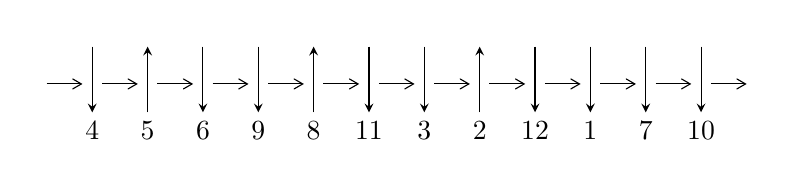
\begin{tikzpicture}[x=20pt, y=17pt]
	% nodes
	\node (C0) at (0, 0) {};
	\node (C1) at (1, 0) {};
	\node (C1U) at (1, +1) {};
	\node (C1D) at (1, -1) {4};

	\node (C2) at (2, 0) {};
	\node (C2U) at (2, +1) {};
	\node (C2D) at (2, -1) {5};

	\node (C3) at (3, 0) {};
	\node (C3U) at (3, +1) {};
	\node (C3D) at (3, -1) {6};

	\node (C4) at (4, 0) {};
	\node (C4U) at (4, +1) {};
	\node (C4D) at (4, -1) {9};

	\node (C5) at (5, 0) {};
	\node (C5U) at (5, +1) {};
	\node (C5D) at (5, -1) {8};

	\node (C6) at (6, 0) {};
	\node (C6U) at (6, +1) {};
	\node (C6D) at (6, -1) {11};

	\node (C7) at (7, 0) {};
	\node (C7U) at (7, +1) {};
	\node (C7D) at (7, -1) {3};

	\node (C8) at (8, 0) {};
	\node (C8U) at (8, +1) {};
	\node (C8D) at (8, -1) {2};

	\node (C9) at (9, 0) {};
	\node (C9U) at (9, +1) {};
	\node (C9D) at (9, -1) {12};

	\node (C10) at (10, 0) {};
	\node (C10U) at (10, +1) {};
	\node (C10D) at (10, -1) {1};

	\node (C11) at (11, 0) {};
	\node (C11U) at (11, +1) {};
	\node (C11D) at (11, -1) {7};

	\node (C12) at (12, 0) {};
	\node (C12U) at (12, +1) {};
	\node (C12D) at (12, -1) {10};
	\node (C13) at (13, 0) {};

	% arrows
	\draw[->,>={angle 60}]
	(C0) edge (C1) (C1) edge (C2) (C2) edge (C3) (C3) edge (C4) (C4) edge (C5) (C5) edge (C6) (C6) edge (C7) (C7) edge (C8) (C8) edge (C9) (C9) edge (C10) (C10) edge (C11) (C11) edge (C12) (C12) edge (C13) ;	\draw[->,>=stealth]
	(C1U) edge (C1D) (C2D) edge (C2U) (C3U) edge (C3D) (C4U) edge (C4D) (C5D) edge (C5U) (C6U) edge (C6D) (C7U) edge (C7D) (C8D) edge (C8U) (C9U) edge (C9D) (C10U) edge (C10D) (C11U) edge (C11D) (C12U) edge (C12D) ;
	\end{tikzpicture} \\
\hhline{~~} \\& 
\textbf{Solving Sequence} \\ \cline{2-2} 
 &
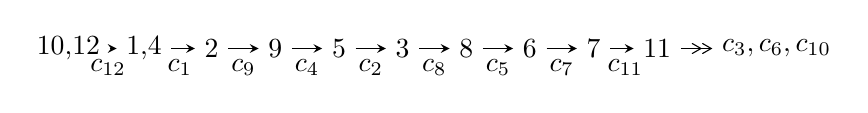
\begin{tikzpicture}[x=23pt, y=7pt]
	% node
	\node (A0) at (-1/8, 0) {10,12};
	\node (A1) at (17/16, 0) {1,4};
	\node (A2) at (17/8, 0) {2};
	\node (A3) at (25/8, 0) {9};
	\node (A4) at (33/8, 0) {5};
	\node (A5) at (41/8, 0) {3};
	\node (A6) at (49/8, 0) {8};
	\node (A7) at (57/8, 0) {6};
	\node (A8) at (65/8, 0) {7};
	\node (A9) at (73/8, 0) {11};
	\node (C1) at (1/2, -1) {$c_{12}$};
	\node (C2) at (13/8, -1) {$c_{1}$};
	\node (C3) at (21/8, -1) {$c_{9}$};
	\node (C4) at (29/8, -1) {$c_{4}$};
	\node (C5) at (37/8, -1) {$c_{2}$};
	\node (C6) at (45/8, -1) {$c_{8}$};
	\node (C7) at (53/8, -1) {$c_{5}$};
	\node (C8) at (61/8, -1) {$c_{7}$};
	\node (C9) at (69/8, -1) {$c_{11}$};
	\node (A10) at (11, 0) {$c_{3},c_{6},c_{10}$};

	% edge
	\draw[->,>=stealth]	
	(A0) edge (A1) (A1) edge (A2) (A2) edge (A3) (A3) edge (A4) (A4) edge (A5) (A5) edge (A6) (A6) edge (A7) (A7) edge (A8) (A8) edge (A9) ;
	\draw[->>,>={angle 60}]	
	(A9) edge (A10);
\end{tikzpicture} \\ 

\end{tabular} \\

\footnotetext{
The image of knot diagram is generated by the software ``\textbf{Draw programme}" developed by Andrew Bartholomew(\url{http://www.layer8.co.uk/maths/draw/index.htm\#Running-draw}), where we modified some parts for our purpose(\url{https://github.com/CATsTAILs/LinksPainter}).
}\phantom \\ \newline 
\centering \textbf{Ideals for irreducible components\footnotemark of $X_{\text{par}}$} 
 
\begin{align*}
I^u_{1}&=\langle 
-7.46655\times10^{73} u^{66}+4.19280\times10^{74} u^{65}+\cdots+5.68441\times10^{73} b+8.22113\times10^{74},\\
\phantom{I^u_{1}}&\phantom{= \langle  }-6.82885\times10^{73} u^{66}+3.74607\times10^{74} u^{65}+\cdots+5.68441\times10^{73} a+4.88086\times10^{74},\\
\phantom{I^u_{1}}&\phantom{= \langle  }u^{67}-7 u^{66}+\cdots+17 u+16\rangle \\
I^u_{2}&=\langle 
-4.31286\times10^{18} a u^{45}+7.66921\times10^{18} u^{45}+\cdots+2.80217\times10^{18} a-5.40388\times10^{18},\\
\phantom{I^u_{2}}&\phantom{= \langle  }4276100239374611 u^{45} a+1318919595635818 u^{45}+\cdots-2872520987122649 a-510440857054024,\\
\phantom{I^u_{2}}&\phantom{= \langle  }u^{46}-5 u^{45}+\cdots+u+1\rangle \\
I^u_{3}&=\langle 
u^{20}-8 u^{19}+\cdots+b-4 u,\;3 u^{20}-12 u^{19}+\cdots+a+3,\;u^{21}-4 u^{20}+\cdots- u-1\rangle \\
I^u_{4}&=\langle 
4 a^3-7 a^2+b+6 a-3,\;4 a^4-7 a^3+7 a^2-4 a+1,\;u+1\rangle \\
I^u_{5}&=\langle 
a^5-5 a^4+13 a^3-16 a^2+b+11 a-4,\;a^6-5 a^5+13 a^4-16 a^3+12 a^2-5 a+1,\;u+1\rangle \\
I^u_{6}&=\langle 
- a u+b- a-1,\;a^2+2 a u- a-3 u+6,\;u^2- u-1\rangle \\
\\
\end{align*}
\raggedright * 6 irreducible components of $\dim_{\mathbb{C}}=0$, with total 194 representations.\\
\footnotetext{All coefficients of polynomials are rational numbers. But the coefficients are sometimes approximated in decimal forms when there is not enough margin.}
\newpage
\renewcommand{\arraystretch}{1}
\centering \section*{I. $I^u_{1}= \langle -7.47\times10^{73} u^{66}+4.19\times10^{74} u^{65}+\cdots+5.68\times10^{73} b+8.22\times10^{74},\;-6.83\times10^{73} u^{66}+3.75\times10^{74} u^{65}+\cdots+5.68\times10^{73} a+4.88\times10^{74},\;u^{67}-7 u^{66}+\cdots+17 u+16 \rangle$}
\flushleft \textbf{(i) Arc colorings}\\
\begin{tabular}{m{7pt} m{180pt} m{7pt} m{180pt} }
\flushright $a_{10}=$&$\begin{pmatrix}0\\u\end{pmatrix}$ \\
\flushright $a_{12}=$&$\begin{pmatrix}1\\0\end{pmatrix}$ \\
\flushright $a_{1}=$&$\begin{pmatrix}1\\u^2\end{pmatrix}$ \\
\flushright $a_{4}=$&$\begin{pmatrix}1.20133 u^{66}-6.59007 u^{65}+\cdots-8.38458 u-8.58640\\1.31351 u^{66}-7.37596 u^{65}+\cdots-28.0095 u-14.4626\end{pmatrix}$ \\
\flushright $a_{2}=$&$\begin{pmatrix}3.37831 u^{66}-18.7956 u^{65}+\cdots-63.1226 u-34.2832\\1.97158 u^{66}-10.8079 u^{65}+\cdots-34.5481 u-19.6508\end{pmatrix}$ \\
\flushright $a_{9}=$&$\begin{pmatrix}u\\u\end{pmatrix}$ \\
\flushright $a_{5}=$&$\begin{pmatrix}1.43693 u^{66}-7.65419 u^{65}+\cdots-6.59990 u-8.59606\\1.54912 u^{66}-8.44009 u^{65}+\cdots-26.2248 u-14.4723\end{pmatrix}$ \\
\flushright $a_{3}=$&$\begin{pmatrix}2.78686 u^{66}-15.6625 u^{65}+\cdots-51.4076 u-30.4248\\1.70541 u^{66}-9.35021 u^{65}+\cdots-30.1704 u-16.9114\end{pmatrix}$ \\
\flushright $a_{8}=$&$\begin{pmatrix}-2.88579 u^{66}+16.9817 u^{65}+\cdots+66.6836 u+38.9741\\-0.883475 u^{66}+5.46866 u^{65}+\cdots+30.5641 u+14.4408\end{pmatrix}$ \\
\flushright $a_{6}=$&$\begin{pmatrix}-1.59108 u^{66}+8.68445 u^{65}+\cdots+35.8380 u+17.6639\\-1.23122 u^{66}+6.72157 u^{65}+\cdots+18.6619 u+12.2584\end{pmatrix}$ \\
\flushright $a_{7}=$&$\begin{pmatrix}2.65000 u^{66}-15.0717 u^{65}+\cdots-65.4616 u-33.0722\\0.963019 u^{66}-5.68222 u^{65}+\cdots-23.4083 u-13.2523\end{pmatrix}$ \\
\flushright $a_{11}=$&$\begin{pmatrix}- u\\- u^3+u\end{pmatrix}$\\&\end{tabular}
\flushleft \textbf{(ii) Obstruction class $= -1$}\\~\\
\flushleft \textbf{(iii) Cusp Shapes $= -2.97364 u^{66}+17.8037 u^{65}+\cdots+63.3507 u+35.1757$}\\~\\
\newpage\renewcommand{\arraystretch}{1}
\flushleft \textbf{(iv) u-Polynomials at the component}\newline \\
\begin{tabular}{m{50pt}|m{274pt}}
Crossings & \hspace{64pt}u-Polynomials at each crossing \\
\hline $$\begin{aligned}c_{1},c_{3}\end{aligned}$$&$\begin{aligned}
&u^{67}+10 u^{66}+\cdots+102 u-1
\end{aligned}$\\
\hline $$\begin{aligned}c_{2}\end{aligned}$$&$\begin{aligned}
&u^{67}+37 u^{66}+\cdots+52 u+4
\end{aligned}$\\
\hline $$\begin{aligned}c_{4},c_{7}\end{aligned}$$&$\begin{aligned}
&u^{67}+5 u^{65}+\cdots-4 u+1
\end{aligned}$\\
\hline $$\begin{aligned}c_{5},c_{8}\end{aligned}$$&$\begin{aligned}
&u^{67}+u^{66}+\cdots+5 u+1
\end{aligned}$\\
\hline $$\begin{aligned}c_{6},c_{11}\end{aligned}$$&$\begin{aligned}
&u^{67}-5 u^{66}+\cdots-736 u+256
\end{aligned}$\\
\hline $$\begin{aligned}c_{9},c_{10},c_{12}\end{aligned}$$&$\begin{aligned}
&u^{67}-7 u^{66}+\cdots+17 u+16
\end{aligned}$\\
\hline
\end{tabular}\\~\\
\newpage\renewcommand{\arraystretch}{1}
\flushleft \textbf{(v) Riley Polynomials at the component}\newline \\
\begin{tabular}{m{50pt}|m{274pt}}
Crossings & \hspace{64pt}Riley Polynomials at each crossing \\
\hline $$\begin{aligned}c_{1},c_{3}\end{aligned}$$&$\begin{aligned}
&y^{67}-34 y^{66}+\cdots+7148 y-1
\end{aligned}$\\
\hline $$\begin{aligned}c_{2}\end{aligned}$$&$\begin{aligned}
&y^{67}- y^{66}+\cdots+1096 y-16
\end{aligned}$\\
\hline $$\begin{aligned}c_{4},c_{7}\end{aligned}$$&$\begin{aligned}
&y^{67}+10 y^{66}+\cdots+40 y-1
\end{aligned}$\\
\hline $$\begin{aligned}c_{5},c_{8}\end{aligned}$$&$\begin{aligned}
&y^{67}+29 y^{66}+\cdots-69 y-1
\end{aligned}$\\
\hline $$\begin{aligned}c_{6},c_{11}\end{aligned}$$&$\begin{aligned}
&y^{67}-27 y^{66}+\cdots+947200 y-65536
\end{aligned}$\\
\hline $$\begin{aligned}c_{9},c_{10},c_{12}\end{aligned}$$&$\begin{aligned}
&y^{67}-59 y^{66}+\cdots-10527 y-256
\end{aligned}$\\
\hline
\end{tabular}\\~\\
\newpage\flushleft \textbf{(vi) Complex Volumes and Cusp Shapes}
$$\begin{array}{c|c|c}  
\text{Solutions to }I^u_{1}& \I (\text{vol} + \sqrt{-1}CS) & \text{Cusp shape}\\
 \hline 
\begin{aligned}
u &= -0.886040 + 0.462607 I \\
a &= \phantom{-}0.418801 - 0.553515 I \\
b &= \phantom{-}0.941164 + 0.197930 I\end{aligned}
 & -3.77727 - 2.29823 I & \phantom{-0.000000 } 0 \\ \hline\begin{aligned}
u &= -0.886040 - 0.462607 I \\
a &= \phantom{-}0.418801 + 0.553515 I \\
b &= \phantom{-}0.941164 - 0.197930 I\end{aligned}
 & -3.77727 + 2.29823 I & \phantom{-0.000000 } 0 \\ \hline\begin{aligned}
u &= -0.506108 + 0.879870 I \\
a &= \phantom{-}0.103195 + 0.584858 I \\
b &= -0.095104 - 0.358363 I\end{aligned}
 & -2.67608 - 0.95592 I & \phantom{-0.000000 } 0 \\ \hline\begin{aligned}
u &= -0.506108 - 0.879870 I \\
a &= \phantom{-}0.103195 - 0.584858 I \\
b &= -0.095104 + 0.358363 I\end{aligned}
 & -2.67608 + 0.95592 I & \phantom{-0.000000 } 0 \\ \hline\begin{aligned}
u &= -0.278352 + 0.927953 I \\
a &= \phantom{-}0.381479 + 0.825242 I \\
b &= -1.177430 + 0.199299 I\end{aligned}
 & -0.2794 + 15.6078 I & -6.00000 - 9.90214 I \\ \hline\begin{aligned}
u &= -0.278352 - 0.927953 I \\
a &= \phantom{-}0.381479 - 0.825242 I \\
b &= -1.177430 - 0.199299 I\end{aligned}
 & -0.2794 - 15.6078 I & -6.00000 + 9.90214 I \\ \hline\begin{aligned}
u &= -0.875010 + 0.359675 I \\
a &= \phantom{-}0.086232 - 0.705853 I \\
b &= \phantom{-}0.651120 - 0.766803 I\end{aligned}
 & -3.78014 + 1.26212 I & -17.5567 - 2.3807 I \\ \hline\begin{aligned}
u &= -0.875010 - 0.359675 I \\
a &= \phantom{-}0.086232 + 0.705853 I \\
b &= \phantom{-}0.651120 + 0.766803 I\end{aligned}
 & -3.78014 - 1.26212 I & -17.5567 + 2.3807 I \\ \hline\begin{aligned}
u &= -0.832278 + 0.744916 I \\
a &= \phantom{-}0.307640 + 0.044559 I \\
b &= -0.719105 - 0.118462 I\end{aligned}
 & -3.66147 + 6.63575 I & \phantom{-0.000000 } 0 \\ \hline\begin{aligned}
u &= -0.832278 - 0.744916 I \\
a &= \phantom{-}0.307640 - 0.044559 I \\
b &= -0.719105 + 0.118462 I\end{aligned}
 & -3.66147 - 6.63575 I & \phantom{-0.000000 } 0\\
 \hline 
 \end{array}$$\newpage$$\begin{array}{c|c|c}  
\text{Solutions to }I^u_{1}& \I (\text{vol} + \sqrt{-1}CS) & \text{Cusp shape}\\
 \hline 
\begin{aligned}
u &= \phantom{-}1.146600 + 0.015974 I \\
a &= \phantom{-}0.236410 - 0.731304 I \\
b &= -0.179252 + 0.333247 I\end{aligned}
 & \phantom{-}0.57345 + 7.56399 I & \phantom{-0.000000 } 0 \\ \hline\begin{aligned}
u &= \phantom{-}1.146600 - 0.015974 I \\
a &= \phantom{-}0.236410 + 0.731304 I \\
b &= -0.179252 - 0.333247 I\end{aligned}
 & \phantom{-}0.57345 - 7.56399 I & \phantom{-0.000000 } 0 \\ \hline\begin{aligned}
u &= -0.265956 + 0.807155 I \\
a &= -0.144674 - 1.268960 I \\
b &= \phantom{-}0.774720 - 0.398888 I\end{aligned}
 & -1.83450 + 6.83794 I & -13.0499 - 9.4798 I \\ \hline\begin{aligned}
u &= -0.265956 - 0.807155 I \\
a &= -0.144674 + 1.268960 I \\
b &= \phantom{-}0.774720 + 0.398888 I\end{aligned}
 & -1.83450 - 6.83794 I & -13.0499 + 9.4798 I \\ \hline\begin{aligned}
u &= -0.142952 + 0.833197 I \\
a &= \phantom{-}0.393388 - 0.285156 I \\
b &= \phantom{-}0.717234 - 0.035393 I\end{aligned}
 & -1.24487 + 2.78705 I & -11.56898 - 3.57731 I \\ \hline\begin{aligned}
u &= -0.142952 - 0.833197 I \\
a &= \phantom{-}0.393388 + 0.285156 I \\
b &= \phantom{-}0.717234 + 0.035393 I\end{aligned}
 & -1.24487 - 2.78705 I & -11.56898 + 3.57731 I \\ \hline\begin{aligned}
u &= -1.151610 + 0.247358 I \\
a &= \phantom{-}1.093750 + 0.479916 I \\
b &= \phantom{-}1.326200 - 0.169578 I\end{aligned}
 & -0.874218 + 1.068790 I & \phantom{-0.000000 } 0 \\ \hline\begin{aligned}
u &= -1.151610 - 0.247358 I \\
a &= \phantom{-}1.093750 - 0.479916 I \\
b &= \phantom{-}1.326200 + 0.169578 I\end{aligned}
 & -0.874218 - 1.068790 I & \phantom{-0.000000 } 0 \\ \hline\begin{aligned}
u &= -1.003220 + 0.631301 I \\
a &= \phantom{-}0.066674 + 0.801201 I \\
b &= -0.139183 - 0.463104 I\end{aligned}
 & -2.46151 - 10.19180 I & \phantom{-0.000000 } 0 \\ \hline\begin{aligned}
u &= -1.003220 - 0.631301 I \\
a &= \phantom{-}0.066674 - 0.801201 I \\
b &= -0.139183 + 0.463104 I\end{aligned}
 & -2.46151 + 10.19180 I & \phantom{-0.000000 } 0\\
 \hline 
 \end{array}$$\newpage$$\begin{array}{c|c|c}  
\text{Solutions to }I^u_{1}& \I (\text{vol} + \sqrt{-1}CS) & \text{Cusp shape}\\
 \hline 
\begin{aligned}
u &= \phantom{-}0.868429 + 0.825439 I \\
a &= \phantom{-}0.178701 + 0.010283 I \\
b &= -0.151600 + 0.224746 I\end{aligned}
 & \phantom{-}4.21754 - 3.05286 I & \phantom{-0.000000 } 0 \\ \hline\begin{aligned}
u &= \phantom{-}0.868429 - 0.825439 I \\
a &= \phantom{-}0.178701 - 0.010283 I \\
b &= -0.151600 - 0.224746 I\end{aligned}
 & \phantom{-}4.21754 + 3.05286 I & \phantom{-0.000000 } 0 \\ \hline\begin{aligned}
u &= -1.226260 + 0.017383 I \\
a &= -2.80177 + 1.01170 I \\
b &= -3.10614 + 1.95095 I\end{aligned}
 & -4.09165 + 0.04865 I & \phantom{-0.000000 } 0 \\ \hline\begin{aligned}
u &= -1.226260 - 0.017383 I \\
a &= -2.80177 - 1.01170 I \\
b &= -3.10614 - 1.95095 I\end{aligned}
 & -4.09165 - 0.04865 I & \phantom{-0.000000 } 0 \\ \hline\begin{aligned}
u &= \phantom{-}0.514220 + 0.564393 I \\
a &= -0.277985 - 0.852832 I \\
b &= -0.077903 + 0.542054 I\end{aligned}
 & \phantom{-}1.47490 + 6.03278 I & -3.03499 - 7.78090 I \\ \hline\begin{aligned}
u &= \phantom{-}0.514220 - 0.564393 I \\
a &= -0.277985 + 0.852832 I \\
b &= -0.077903 - 0.542054 I\end{aligned}
 & \phantom{-}1.47490 - 6.03278 I & -3.03499 + 7.78090 I \\ \hline\begin{aligned}
u &= \phantom{-}0.317644 + 0.657692 I \\
a &= \phantom{-}0.923425 - 0.718468 I \\
b &= -0.990234 - 0.352466 I\end{aligned}
 & \phantom{-}2.11508 - 9.83520 I & -3.28213 + 7.19382 I \\ \hline\begin{aligned}
u &= \phantom{-}0.317644 - 0.657692 I \\
a &= \phantom{-}0.923425 + 0.718468 I \\
b &= -0.990234 + 0.352466 I\end{aligned}
 & \phantom{-}2.11508 + 9.83520 I & -3.28213 - 7.19382 I \\ \hline\begin{aligned}
u &= -1.267820 + 0.254906 I \\
a &= -0.98278 - 1.28187 I \\
b &= -1.23559 - 1.32066 I\end{aligned}
 & -4.47405 + 1.01497 I & \phantom{-0.000000 } 0 \\ \hline\begin{aligned}
u &= -1.267820 - 0.254906 I \\
a &= -0.98278 + 1.28187 I \\
b &= -1.23559 + 1.32066 I\end{aligned}
 & -4.47405 - 1.01497 I & \phantom{-0.000000 } 0\\
 \hline 
 \end{array}$$\newpage$$\begin{array}{c|c|c}  
\text{Solutions to }I^u_{1}& \I (\text{vol} + \sqrt{-1}CS) & \text{Cusp shape}\\
 \hline 
\begin{aligned}
u &= -0.122225 + 0.694677 I \\
a &= \phantom{-}0.507052 - 0.261280 I \\
b &= -0.863507 - 0.202693 I\end{aligned}
 & \phantom{-}2.18927 + 2.39577 I & -0.67460 - 3.37107 I \\ \hline\begin{aligned}
u &= -0.122225 - 0.694677 I \\
a &= \phantom{-}0.507052 + 0.261280 I \\
b &= -0.863507 + 0.202693 I\end{aligned}
 & \phantom{-}2.18927 - 2.39577 I & -0.67460 + 3.37107 I \\ \hline\begin{aligned}
u &= \phantom{-}1.308110 + 0.162425 I \\
a &= \phantom{-}0.626403 + 0.525881 I \\
b &= \phantom{-}1.097540 - 0.180102 I\end{aligned}
 & -4.15383 - 0.16010 I & \phantom{-0.000000 } 0 \\ \hline\begin{aligned}
u &= \phantom{-}1.308110 - 0.162425 I \\
a &= \phantom{-}0.626403 - 0.525881 I \\
b &= \phantom{-}1.097540 + 0.180102 I\end{aligned}
 & -4.15383 + 0.16010 I & \phantom{-0.000000 } 0 \\ \hline\begin{aligned}
u &= -0.650492\phantom{ +0.000000I} \\
a &= \phantom{-}0.859311\phantom{ +0.000000I} \\
b &= \phantom{-}0.351682\phantom{ +0.000000I}\end{aligned}
 & -1.00288\phantom{ +0.000000I} & -10.0410\phantom{ +0.000000I} \\ \hline\begin{aligned}
u &= -1.334120 + 0.204364 I \\
a &= -2.54568 - 0.16258 I \\
b &= -3.25877 + 0.06740 I\end{aligned}
 & -4.75755 + 4.80110 I & \phantom{-0.000000 } 0 \\ \hline\begin{aligned}
u &= -1.334120 - 0.204364 I \\
a &= -2.54568 + 0.16258 I \\
b &= -3.25877 - 0.06740 I\end{aligned}
 & -4.75755 - 4.80110 I & \phantom{-0.000000 } 0 \\ \hline\begin{aligned}
u &= -0.297590 + 0.569032 I \\
a &= -0.388782 + 0.838417 I \\
b &= \phantom{-}1.67541 + 0.17339 I\end{aligned}
 & -1.93809 + 1.60095 I & -10.43691 - 4.02924 I \\ \hline\begin{aligned}
u &= -0.297590 - 0.569032 I \\
a &= -0.388782 - 0.838417 I \\
b &= \phantom{-}1.67541 - 0.17339 I\end{aligned}
 & -1.93809 - 1.60095 I & -10.43691 + 4.02924 I \\ \hline\begin{aligned}
u &= -0.363048 + 0.527813 I \\
a &= \phantom{-}0.67980 - 1.94335 I \\
b &= -0.054527 - 0.387963 I\end{aligned}
 & -2.13919 + 1.55825 I & -11.25159 - 5.43160 I\\
 \hline 
 \end{array}$$\newpage$$\begin{array}{c|c|c}  
\text{Solutions to }I^u_{1}& \I (\text{vol} + \sqrt{-1}CS) & \text{Cusp shape}\\
 \hline 
\begin{aligned}
u &= -0.363048 - 0.527813 I \\
a &= \phantom{-}0.67980 + 1.94335 I \\
b &= -0.054527 + 0.387963 I\end{aligned}
 & -2.13919 - 1.55825 I & -11.25159 + 5.43160 I \\ \hline\begin{aligned}
u &= \phantom{-}1.342900 + 0.275476 I \\
a &= \phantom{-}0.895399 - 0.647673 I \\
b &= \phantom{-}1.231760 + 0.093797 I\end{aligned}
 & -2.43663 - 5.90398 I & \phantom{-0.000000 } 0 \\ \hline\begin{aligned}
u &= \phantom{-}1.342900 - 0.275476 I \\
a &= \phantom{-}0.895399 + 0.647673 I \\
b &= \phantom{-}1.231760 - 0.093797 I\end{aligned}
 & -2.43663 + 5.90398 I & \phantom{-0.000000 } 0 \\ \hline\begin{aligned}
u &= \phantom{-}1.41253 + 0.22914 I \\
a &= -1.74771 + 0.52569 I \\
b &= -2.18934 - 0.54716 I\end{aligned}
 & -7.40801 - 4.57388 I & \phantom{-0.000000 } 0 \\ \hline\begin{aligned}
u &= \phantom{-}1.41253 - 0.22914 I \\
a &= -1.74771 - 0.52569 I \\
b &= -2.18934 + 0.54716 I\end{aligned}
 & -7.40801 + 4.57388 I & \phantom{-0.000000 } 0 \\ \hline\begin{aligned}
u &= \phantom{-}1.38655 + 0.37104 I \\
a &= -1.078820 + 0.668747 I \\
b &= -1.43331 + 0.46079 I\end{aligned}
 & -6.09824 - 7.18020 I & \phantom{-0.000000 } 0 \\ \hline\begin{aligned}
u &= \phantom{-}1.38655 - 0.37104 I \\
a &= -1.078820 - 0.668747 I \\
b &= -1.43331 - 0.46079 I\end{aligned}
 & -6.09824 + 7.18020 I & \phantom{-0.000000 } 0 \\ \hline\begin{aligned}
u &= \phantom{-}1.42617 + 0.19546 I \\
a &= -0.990215 + 0.549897 I \\
b &= -1.49974 + 1.39131 I\end{aligned}
 & -7.87593 - 4.21311 I & \phantom{-0.000000 } 0 \\ \hline\begin{aligned}
u &= \phantom{-}1.42617 - 0.19546 I \\
a &= -0.990215 - 0.549897 I \\
b &= -1.49974 - 1.39131 I\end{aligned}
 & -7.87593 + 4.21311 I & \phantom{-0.000000 } 0 \\ \hline\begin{aligned}
u &= -1.42366 + 0.26282 I \\
a &= \phantom{-}2.21278 + 0.02414 I \\
b &= \phantom{-}3.06613 - 0.66738 I\end{aligned}
 & -3.44703 + 13.22340 I & \phantom{-0.000000 } 0\\
 \hline 
 \end{array}$$\newpage$$\begin{array}{c|c|c}  
\text{Solutions to }I^u_{1}& \I (\text{vol} + \sqrt{-1}CS) & \text{Cusp shape}\\
 \hline 
\begin{aligned}
u &= -1.42366 - 0.26282 I \\
a &= \phantom{-}2.21278 - 0.02414 I \\
b &= \phantom{-}3.06613 + 0.66738 I\end{aligned}
 & -3.44703 - 13.22340 I & \phantom{-0.000000 } 0 \\ \hline\begin{aligned}
u &= \phantom{-}1.41803 + 0.32540 I \\
a &= -2.05092 + 0.35648 I \\
b &= -2.83519 + 0.16768 I\end{aligned}
 & -7.19836 - 10.93070 I & \phantom{-0.000000 } 0 \\ \hline\begin{aligned}
u &= \phantom{-}1.41803 - 0.32540 I \\
a &= -2.05092 - 0.35648 I \\
b &= -2.83519 - 0.16768 I\end{aligned}
 & -7.19836 + 10.93070 I & \phantom{-0.000000 } 0 \\ \hline\begin{aligned}
u &= \phantom{-}0.077770 + 0.518056 I \\
a &= -0.54086 + 1.77842 I \\
b &= \phantom{-}0.801606 + 0.510059 I\end{aligned}
 & -0.26465 - 2.13116 I & -8.00844 + 3.42216 I \\ \hline\begin{aligned}
u &= \phantom{-}0.077770 - 0.518056 I \\
a &= -0.54086 - 1.77842 I \\
b &= \phantom{-}0.801606 - 0.510059 I\end{aligned}
 & -0.26465 + 2.13116 I & -8.00844 - 3.42216 I \\ \hline\begin{aligned}
u &= \phantom{-}1.48184 + 0.01796 I \\
a &= -1.88623 + 0.56334 I \\
b &= -2.49946 + 0.63940 I\end{aligned}
 & -11.54390 + 1.53289 I & \phantom{-0.000000 } 0 \\ \hline\begin{aligned}
u &= \phantom{-}1.48184 - 0.01796 I \\
a &= -1.88623 - 0.56334 I \\
b &= -2.49946 - 0.63940 I\end{aligned}
 & -11.54390 - 1.53289 I & \phantom{-0.000000 } 0 \\ \hline\begin{aligned}
u &= -1.48064 + 0.12268 I \\
a &= \phantom{-}0.960629 + 0.677197 I \\
b &= \phantom{-}1.60297 + 1.04822 I\end{aligned}
 & -5.25353 - 3.65413 I & \phantom{-0.000000 } 0 \\ \hline\begin{aligned}
u &= -1.48064 - 0.12268 I \\
a &= \phantom{-}0.960629 - 0.677197 I \\
b &= \phantom{-}1.60297 - 1.04822 I\end{aligned}
 & -5.25353 + 3.65413 I & \phantom{-0.000000 } 0 \\ \hline\begin{aligned}
u &= \phantom{-}1.44769 + 0.37948 I \\
a &= \phantom{-}2.01395 - 0.39710 I \\
b &= \phantom{-}2.93042 + 0.30305 I\end{aligned}
 & -5.7776 - 20.3102 I & \phantom{-0.000000 } 0\\
 \hline 
 \end{array}$$\newpage$$\begin{array}{c|c|c}  
\text{Solutions to }I^u_{1}& \I (\text{vol} + \sqrt{-1}CS) & \text{Cusp shape}\\
 \hline 
\begin{aligned}
u &= \phantom{-}1.44769 - 0.37948 I \\
a &= \phantom{-}2.01395 + 0.39710 I \\
b &= \phantom{-}2.93042 - 0.30305 I\end{aligned}
 & -5.7776 + 20.3102 I & \phantom{-0.000000 } 0 \\ \hline\begin{aligned}
u &= \phantom{-}1.50160 + 0.27397 I \\
a &= \phantom{-}0.892084 - 0.367176 I \\
b &= \phantom{-}1.66203 - 0.53253 I\end{aligned}
 & -9.25323 - 3.05507 I & \phantom{-0.000000 } 0 \\ \hline\begin{aligned}
u &= \phantom{-}1.50160 - 0.27397 I \\
a &= \phantom{-}0.892084 + 0.367176 I \\
b &= \phantom{-}1.66203 + 0.53253 I\end{aligned}
 & -9.25323 + 3.05507 I & \phantom{-0.000000 } 0 \\ \hline\begin{aligned}
u &= \phantom{-}1.57951 + 0.06444 I \\
a &= \phantom{-}1.49720 + 0.37848 I \\
b &= \phantom{-}2.31797 + 0.90383 I\end{aligned}
 & -12.2490 - 9.1394 I & \phantom{-0.000000 } 0 \\ \hline\begin{aligned}
u &= \phantom{-}1.57951 - 0.06444 I \\
a &= \phantom{-}1.49720 - 0.37848 I \\
b &= \phantom{-}2.31797 - 0.90383 I\end{aligned}
 & -12.2490 + 9.1394 I & \phantom{-0.000000 } 0 \\ \hline\begin{aligned}
u &= \phantom{-}0.052527 + 0.206865 I \\
a &= \phantom{-}2.37554 + 2.38725 I \\
b &= \phantom{-}0.408286 - 0.391016 I\end{aligned}
 & -0.97444 + 1.07725 I & -5.67594 - 4.49690 I \\ \hline\begin{aligned}
u &= \phantom{-}0.052527 - 0.206865 I \\
a &= \phantom{-}2.37554 - 2.38725 I \\
b &= \phantom{-}0.408286 + 0.391016 I\end{aligned}
 & -0.97444 - 1.07725 I & -5.67594 + 4.49690 I\\
 \hline 
 \end{array}$$\newpage\newpage\renewcommand{\arraystretch}{1}
\centering \section*{II. $I^u_{2}= \langle -4.31\times10^{18} a u^{45}+7.67\times10^{18} u^{45}+\cdots+2.80\times10^{18} a-5.40\times10^{18},\;4.28\times10^{15} a u^{45}+1.32\times10^{15} u^{45}+\cdots-2.87\times10^{15} a-5.10\times10^{14},\;u^{46}-5 u^{45}+\cdots+u+1 \rangle$}
\flushleft \textbf{(i) Arc colorings}\\
\begin{tabular}{m{7pt} m{180pt} m{7pt} m{180pt} }
\flushright $a_{10}=$&$\begin{pmatrix}0\\u\end{pmatrix}$ \\
\flushright $a_{12}=$&$\begin{pmatrix}1\\0\end{pmatrix}$ \\
\flushright $a_{1}=$&$\begin{pmatrix}1\\u^2\end{pmatrix}$ \\
\flushright $a_{4}=$&$\begin{pmatrix}a\\7.26494 a u^{45}-12.9187 u^{45}+\cdots-4.72021 a+9.10275\end{pmatrix}$ \\
\flushright $a_{2}=$&$\begin{pmatrix}10.0594 a u^{45}+15.4174 u^{45}+\cdots-8.05021 a-12.4526\\6.68466 a u^{45}+7.33727 u^{45}+\cdots-5.87490 a-7.18934\end{pmatrix}$ \\
\flushright $a_{9}=$&$\begin{pmatrix}u\\u\end{pmatrix}$ \\
\flushright $a_{5}=$&$\begin{pmatrix}-15.9507 a u^{45}+30.4136 u^{45}+\cdots+11.8538 a-20.4155\\-8.68580 a u^{45}+17.4950 u^{45}+\cdots+6.13364 a-11.3128\end{pmatrix}$ \\
\flushright $a_{3}=$&$\begin{pmatrix}-17.5185 a u^{45}+44.1901 u^{45}+\cdots+13.3266 a-31.6617\\-5.57001 a u^{45}+23.9234 u^{45}+\cdots+4.75911 a-17.0092\end{pmatrix}$ \\
\flushright $a_{8}=$&$\begin{pmatrix}-8.81370 a u^{45}-30.2038 u^{45}+\cdots+5.57064 a+20.7364\\-9.90551 a u^{45}-24.5364 u^{45}+\cdots+5.91698 a+16.1933\end{pmatrix}$ \\
\flushright $a_{6}=$&$\begin{pmatrix}16.2495 u^{45}-56.2137 u^{44}+\cdots-20.5991 u-11.7119\\11.5267 u^{45}-40.6880 u^{44}+\cdots-11.8242 u-7.98688\end{pmatrix}$ \\
\flushright $a_{7}=$&$\begin{pmatrix}-26.2810 u^{45}+96.5901 u^{44}+\cdots+38.3673 u+20.9461\\-9.23423 u^{45}+36.1396 u^{44}+\cdots+13.8688 u+8.53396\end{pmatrix}$ \\
\flushright $a_{11}=$&$\begin{pmatrix}- u\\- u^3+u\end{pmatrix}$\\&\end{tabular}
\flushleft \textbf{(ii) Obstruction class $= -1$}\\~\\
\flushleft \textbf{(iii) Cusp Shapes $= -\frac{3565132764588699}{137866554138758} u^{45}+\frac{12143571441573331}{137866554138758} u^{44}+\cdots+\frac{5241235151619549}{137866554138758} u+\frac{692954415625718}{68933277069379}$}\\~\\
\newpage\renewcommand{\arraystretch}{1}
\flushleft \textbf{(iv) u-Polynomials at the component}\newline \\
\begin{tabular}{m{50pt}|m{274pt}}
Crossings & \hspace{64pt}u-Polynomials at each crossing \\
\hline $$\begin{aligned}c_{1},c_{3}\end{aligned}$$&$\begin{aligned}
&u^{92}-6 u^{91}+\cdots+21848 u-4007
\end{aligned}$\\
\hline $$\begin{aligned}c_{2}\end{aligned}$$&$\begin{aligned}
&(u^{46}-22 u^{45}+\cdots+6 u+4)^{2}
\end{aligned}$\\
\hline $$\begin{aligned}c_{4},c_{7}\end{aligned}$$&$\begin{aligned}
&u^{92}+5 u^{91}+\cdots+59081 u-15649
\end{aligned}$\\
\hline $$\begin{aligned}c_{5},c_{8}\end{aligned}$$&$\begin{aligned}
&u^{92}+9 u^{91}+\cdots+9 u+1
\end{aligned}$\\
\hline $$\begin{aligned}c_{6},c_{11}\end{aligned}$$&$\begin{aligned}
&(u^{46}+2 u^{45}+\cdots+12 u-8)^{2}
\end{aligned}$\\
\hline $$\begin{aligned}c_{9},c_{10},c_{12}\end{aligned}$$&$\begin{aligned}
&(u^{46}-5 u^{45}+\cdots+u+1)^{2}
\end{aligned}$\\
\hline
\end{tabular}\\~\\
\newpage\renewcommand{\arraystretch}{1}
\flushleft \textbf{(v) Riley Polynomials at the component}\newline \\
\begin{tabular}{m{50pt}|m{274pt}}
Crossings & \hspace{64pt}Riley Polynomials at each crossing \\
\hline $$\begin{aligned}c_{1},c_{3}\end{aligned}$$&$\begin{aligned}
&y^{92}+26 y^{91}+\cdots-169276944 y+16056049
\end{aligned}$\\
\hline $$\begin{aligned}c_{2}\end{aligned}$$&$\begin{aligned}
&(y^{46}-6 y^{45}+\cdots-460 y+16)^{2}
\end{aligned}$\\
\hline $$\begin{aligned}c_{4},c_{7}\end{aligned}$$&$\begin{aligned}
&y^{92}- y^{91}+\cdots+7756027461 y+244891201
\end{aligned}$\\
\hline $$\begin{aligned}c_{5},c_{8}\end{aligned}$$&$\begin{aligned}
&y^{92}-25 y^{91}+\cdots+5 y+1
\end{aligned}$\\
\hline $$\begin{aligned}c_{6},c_{11}\end{aligned}$$&$\begin{aligned}
&(y^{46}-24 y^{45}+\cdots-464 y+64)^{2}
\end{aligned}$\\
\hline $$\begin{aligned}c_{9},c_{10},c_{12}\end{aligned}$$&$\begin{aligned}
&(y^{46}-43 y^{45}+\cdots+y+1)^{2}
\end{aligned}$\\
\hline
\end{tabular}\\~\\
\newpage\flushleft \textbf{(vi) Complex Volumes and Cusp Shapes}
$$\begin{array}{c|c|c}  
\text{Solutions to }I^u_{2}& \I (\text{vol} + \sqrt{-1}CS) & \text{Cusp shape}\\
 \hline 
\begin{aligned}
u &= -0.301208 + 0.925317 I \\
a &= \phantom{-}0.539502 + 0.595975 I \\
b &= -1.070430 - 0.078921 I\end{aligned}
 & \phantom{-}1.27204 + 7.29420 I & -2.20923 - 9.60817 I \\ \hline\begin{aligned}
u &= -0.301208 + 0.925317 I \\
a &= -0.235983 - 0.541720 I \\
b &= \phantom{-}0.514580 - 0.442022 I\end{aligned}
 & \phantom{-}1.27204 + 7.29420 I & -2.20923 - 9.60817 I \\ \hline\begin{aligned}
u &= -0.301208 - 0.925317 I \\
a &= \phantom{-}0.539502 - 0.595975 I \\
b &= -1.070430 + 0.078921 I\end{aligned}
 & \phantom{-}1.27204 - 7.29420 I & -2.20923 + 9.60817 I \\ \hline\begin{aligned}
u &= -0.301208 - 0.925317 I \\
a &= -0.235983 + 0.541720 I \\
b &= \phantom{-}0.514580 + 0.442022 I\end{aligned}
 & \phantom{-}1.27204 - 7.29420 I & -2.20923 + 9.60817 I \\ \hline\begin{aligned}
u &= -0.722332 + 0.600949 I \\
a &= \phantom{-}0.547852 - 0.821980 I \\
b &= \phantom{-}0.521373 + 0.207530 I\end{aligned}
 & -3.35914 - 1.96952 I & -15.8602 + 4.3814 I \\ \hline\begin{aligned}
u &= -0.722332 + 0.600949 I \\
a &= \phantom{-}0.628225 - 0.570814 I \\
b &= -1.159030 - 0.808305 I\end{aligned}
 & -3.35914 - 1.96952 I & -15.8602 + 4.3814 I \\ \hline\begin{aligned}
u &= -0.722332 - 0.600949 I \\
a &= \phantom{-}0.547852 + 0.821980 I \\
b &= \phantom{-}0.521373 - 0.207530 I\end{aligned}
 & -3.35914 + 1.96952 I & -15.8602 - 4.3814 I \\ \hline\begin{aligned}
u &= -0.722332 - 0.600949 I \\
a &= \phantom{-}0.628225 + 0.570814 I \\
b &= -1.159030 + 0.808305 I\end{aligned}
 & -3.35914 + 1.96952 I & -15.8602 - 4.3814 I \\ \hline\begin{aligned}
u &= -1.069300 + 0.154626 I \\
a &= -0.028114 + 0.733560 I \\
b &= \phantom{-}0.58442 + 1.82190 I\end{aligned}
 & -0.54999 - 3.11732 I & -1.92655 + 7.58795 I \\ \hline\begin{aligned}
u &= -1.069300 + 0.154626 I \\
a &= \phantom{-}4.41452 - 0.50911 I \\
b &= \phantom{-}4.15151 - 0.93227 I\end{aligned}
 & -0.54999 - 3.11732 I & -1.92655 + 7.58795 I\\
 \hline 
 \end{array}$$\newpage$$\begin{array}{c|c|c}  
\text{Solutions to }I^u_{2}& \I (\text{vol} + \sqrt{-1}CS) & \text{Cusp shape}\\
 \hline 
\begin{aligned}
u &= -1.069300 - 0.154626 I \\
a &= -0.028114 - 0.733560 I \\
b &= \phantom{-}0.58442 - 1.82190 I\end{aligned}
 & -0.54999 + 3.11732 I & -1.92655 - 7.58795 I \\ \hline\begin{aligned}
u &= -1.069300 - 0.154626 I \\
a &= \phantom{-}4.41452 + 0.50911 I \\
b &= \phantom{-}4.15151 + 0.93227 I\end{aligned}
 & -0.54999 + 3.11732 I & -1.92655 - 7.58795 I \\ \hline\begin{aligned}
u &= -0.371010 + 0.778352 I \\
a &= -0.335013 - 0.893259 I \\
b &= \phantom{-}0.943969 - 0.589431 I\end{aligned}
 & -2.25962 + 6.70622 I & -12.6754 - 9.2419 I \\ \hline\begin{aligned}
u &= -0.371010 + 0.778352 I \\
a &= \phantom{-}0.37172 + 1.51058 I \\
b &= \phantom{-}0.135168 - 0.591500 I\end{aligned}
 & -2.25962 + 6.70622 I & -12.6754 - 9.2419 I \\ \hline\begin{aligned}
u &= -0.371010 - 0.778352 I \\
a &= -0.335013 + 0.893259 I \\
b &= \phantom{-}0.943969 + 0.589431 I\end{aligned}
 & -2.25962 - 6.70622 I & -12.6754 + 9.2419 I \\ \hline\begin{aligned}
u &= -0.371010 - 0.778352 I \\
a &= \phantom{-}0.37172 - 1.51058 I \\
b &= \phantom{-}0.135168 + 0.591500 I\end{aligned}
 & -2.25962 - 6.70622 I & -12.6754 + 9.2419 I \\ \hline\begin{aligned}
u &= -0.968236 + 0.657208 I \\
a &= \phantom{-}0.385680 + 0.494198 I \\
b &= \phantom{-}0.021923 - 0.727960 I\end{aligned}
 & -0.73382 - 1.83088 I & \phantom{-0.000000 } 0 \\ \hline\begin{aligned}
u &= -0.968236 + 0.657208 I \\
a &= \phantom{-}0.351392 - 0.367182 I \\
b &= \phantom{-}0.216413 + 0.038938 I\end{aligned}
 & -0.73382 - 1.83088 I & \phantom{-0.000000 } 0 \\ \hline\begin{aligned}
u &= -0.968236 - 0.657208 I \\
a &= \phantom{-}0.385680 - 0.494198 I \\
b &= \phantom{-}0.021923 + 0.727960 I\end{aligned}
 & -0.73382 + 1.83088 I & \phantom{-0.000000 } 0 \\ \hline\begin{aligned}
u &= -0.968236 - 0.657208 I \\
a &= \phantom{-}0.351392 + 0.367182 I \\
b &= \phantom{-}0.216413 - 0.038938 I\end{aligned}
 & -0.73382 + 1.83088 I & \phantom{-0.000000 } 0\\
 \hline 
 \end{array}$$\newpage$$\begin{array}{c|c|c}  
\text{Solutions to }I^u_{2}& \I (\text{vol} + \sqrt{-1}CS) & \text{Cusp shape}\\
 \hline 
\begin{aligned}
u &= \phantom{-}1.18912\phantom{ +0.000000I} \\
a &= \phantom{-}0.381769 + 0.593804 I \\
b &= \phantom{-}0.205686 - 0.488546 I\end{aligned}
 & \phantom{-}2.15622\phantom{ +0.000000I} & -11.6170\phantom{ +0.000000I} \\ \hline\begin{aligned}
u &= \phantom{-}1.18912\phantom{ +0.000000I} \\
a &= \phantom{-}0.381769 - 0.593804 I \\
b &= \phantom{-}0.205686 + 0.488546 I\end{aligned}
 & \phantom{-}2.15622\phantom{ +0.000000I} & -11.6170\phantom{ +0.000000I} \\ \hline\begin{aligned}
u &= -1.147130 + 0.330381 I \\
a &= \phantom{-}0.662485 - 0.140870 I \\
b &= \phantom{-}0.941847 - 0.872914 I\end{aligned}
 & -1.02869 + 1.23073 I & \phantom{-0.000000 } 0 \\ \hline\begin{aligned}
u &= -1.147130 + 0.330381 I \\
a &= \phantom{-}1.45074 + 1.11037 I \\
b &= \phantom{-}1.60150 + 0.22264 I\end{aligned}
 & -1.02869 + 1.23073 I & \phantom{-0.000000 } 0 \\ \hline\begin{aligned}
u &= -1.147130 - 0.330381 I \\
a &= \phantom{-}0.662485 + 0.140870 I \\
b &= \phantom{-}0.941847 + 0.872914 I\end{aligned}
 & -1.02869 - 1.23073 I & \phantom{-0.000000 } 0 \\ \hline\begin{aligned}
u &= -1.147130 - 0.330381 I \\
a &= \phantom{-}1.45074 - 1.11037 I \\
b &= \phantom{-}1.60150 - 0.22264 I\end{aligned}
 & -1.02869 - 1.23073 I & \phantom{-0.000000 } 0 \\ \hline\begin{aligned}
u &= -1.209740 + 0.143206 I \\
a &= -0.20791 + 2.25198 I \\
b &= \phantom{-}0.06312 + 1.64377 I\end{aligned}
 & -0.98248 + 4.74267 I & \phantom{-0.000000 } 0 \\ \hline\begin{aligned}
u &= -1.209740 + 0.143206 I \\
a &= -3.71784 + 0.24484 I \\
b &= -4.79294 + 0.94523 I\end{aligned}
 & -0.98248 + 4.74267 I & \phantom{-0.000000 } 0 \\ \hline\begin{aligned}
u &= -1.209740 - 0.143206 I \\
a &= -0.20791 - 2.25198 I \\
b &= \phantom{-}0.06312 - 1.64377 I\end{aligned}
 & -0.98248 - 4.74267 I & \phantom{-0.000000 } 0 \\ \hline\begin{aligned}
u &= -1.209740 - 0.143206 I \\
a &= -3.71784 - 0.24484 I \\
b &= -4.79294 - 0.94523 I\end{aligned}
 & -0.98248 - 4.74267 I & \phantom{-0.000000 } 0\\
 \hline 
 \end{array}$$\newpage$$\begin{array}{c|c|c}  
\text{Solutions to }I^u_{2}& \I (\text{vol} + \sqrt{-1}CS) & \text{Cusp shape}\\
 \hline 
\begin{aligned}
u &= -0.227074 + 0.675918 I \\
a &= -0.04766 - 1.46821 I \\
b &= -1.11495 - 1.22759 I\end{aligned}
 & \phantom{-}1.69571 + 6.30129 I & -2.30828 - 10.19820 I \\ \hline\begin{aligned}
u &= -0.227074 + 0.675918 I \\
a &= -1.29068 - 1.06858 I \\
b &= \phantom{-}0.860694 + 0.064321 I\end{aligned}
 & \phantom{-}1.69571 + 6.30129 I & -2.30828 - 10.19820 I \\ \hline\begin{aligned}
u &= -0.227074 - 0.675918 I \\
a &= -0.04766 + 1.46821 I \\
b &= -1.11495 + 1.22759 I\end{aligned}
 & \phantom{-}1.69571 - 6.30129 I & -2.30828 + 10.19820 I \\ \hline\begin{aligned}
u &= -0.227074 - 0.675918 I \\
a &= -1.29068 + 1.06858 I \\
b &= \phantom{-}0.860694 - 0.064321 I\end{aligned}
 & \phantom{-}1.69571 - 6.30129 I & -2.30828 + 10.19820 I \\ \hline\begin{aligned}
u &= \phantom{-}0.344671 + 0.595078 I \\
a &= \phantom{-}1.103900 - 0.381172 I \\
b &= -0.664606 - 0.215065 I\end{aligned}
 & \phantom{-}3.89027 - 1.72774 I & \phantom{-}3.38137 + 3.27076 I \\ \hline\begin{aligned}
u &= \phantom{-}0.344671 + 0.595078 I \\
a &= -0.612797 - 0.019410 I \\
b &= \phantom{-}0.279786 + 0.632492 I\end{aligned}
 & \phantom{-}3.89027 - 1.72774 I & \phantom{-}3.38137 + 3.27076 I \\ \hline\begin{aligned}
u &= \phantom{-}0.344671 - 0.595078 I \\
a &= \phantom{-}1.103900 + 0.381172 I \\
b &= -0.664606 + 0.215065 I\end{aligned}
 & \phantom{-}3.89027 + 1.72774 I & \phantom{-}3.38137 - 3.27076 I \\ \hline\begin{aligned}
u &= \phantom{-}0.344671 - 0.595078 I \\
a &= -0.612797 + 0.019410 I \\
b &= \phantom{-}0.279786 - 0.632492 I\end{aligned}
 & \phantom{-}3.89027 + 1.72774 I & \phantom{-}3.38137 - 3.27076 I \\ \hline\begin{aligned}
u &= -0.085734 + 0.681652 I \\
a &= \phantom{-}0.963556 - 0.446059 I \\
b &= -0.619372 - 0.367941 I\end{aligned}
 & \phantom{-}2.23568 + 2.45642 I & -0.01179 - 3.81685 I \\ \hline\begin{aligned}
u &= -0.085734 + 0.681652 I \\
a &= \phantom{-}0.126903 - 0.138439 I \\
b &= -1.141800 + 0.059750 I\end{aligned}
 & \phantom{-}2.23568 + 2.45642 I & -0.01179 - 3.81685 I\\
 \hline 
 \end{array}$$\newpage$$\begin{array}{c|c|c}  
\text{Solutions to }I^u_{2}& \I (\text{vol} + \sqrt{-1}CS) & \text{Cusp shape}\\
 \hline 
\begin{aligned}
u &= -0.085734 - 0.681652 I \\
a &= \phantom{-}0.963556 + 0.446059 I \\
b &= -0.619372 + 0.367941 I\end{aligned}
 & \phantom{-}2.23568 - 2.45642 I & -0.01179 + 3.81685 I \\ \hline\begin{aligned}
u &= -0.085734 - 0.681652 I \\
a &= \phantom{-}0.126903 + 0.138439 I \\
b &= -1.141800 - 0.059750 I\end{aligned}
 & \phantom{-}2.23568 - 2.45642 I & -0.01179 + 3.81685 I \\ \hline\begin{aligned}
u &= \phantom{-}1.341210 + 0.248066 I \\
a &= \phantom{-}0.352859 - 0.409330 I \\
b &= \phantom{-}0.589078 + 0.533839 I\end{aligned}
 & -2.27518 - 5.75756 I & \phantom{-0.000000 } 0 \\ \hline\begin{aligned}
u &= \phantom{-}1.341210 + 0.248066 I \\
a &= \phantom{-}1.57949 - 0.74710 I \\
b &= \phantom{-}1.83012 - 0.27573 I\end{aligned}
 & -2.27518 - 5.75756 I & \phantom{-0.000000 } 0 \\ \hline\begin{aligned}
u &= \phantom{-}1.341210 - 0.248066 I \\
a &= \phantom{-}0.352859 + 0.409330 I \\
b &= \phantom{-}0.589078 - 0.533839 I\end{aligned}
 & -2.27518 + 5.75756 I & \phantom{-0.000000 } 0 \\ \hline\begin{aligned}
u &= \phantom{-}1.341210 - 0.248066 I \\
a &= \phantom{-}1.57949 + 0.74710 I \\
b &= \phantom{-}1.83012 + 0.27573 I\end{aligned}
 & -2.27518 + 5.75756 I & \phantom{-0.000000 } 0 \\ \hline\begin{aligned}
u &= \phantom{-}1.352860 + 0.220635 I \\
a &= -0.090295 + 0.166667 I \\
b &= \phantom{-}0.286702 - 1.050280 I\end{aligned}
 & -2.52895 - 0.78794 I & \phantom{-0.000000 } 0 \\ \hline\begin{aligned}
u &= \phantom{-}1.352860 + 0.220635 I \\
a &= \phantom{-}2.25611 + 0.05895 I \\
b &= \phantom{-}2.47483 + 0.22157 I\end{aligned}
 & -2.52895 - 0.78794 I & \phantom{-0.000000 } 0 \\ \hline\begin{aligned}
u &= \phantom{-}1.352860 - 0.220635 I \\
a &= -0.090295 - 0.166667 I \\
b &= \phantom{-}0.286702 + 1.050280 I\end{aligned}
 & -2.52895 + 0.78794 I & \phantom{-0.000000 } 0 \\ \hline\begin{aligned}
u &= \phantom{-}1.352860 - 0.220635 I \\
a &= \phantom{-}2.25611 - 0.05895 I \\
b &= \phantom{-}2.47483 - 0.22157 I\end{aligned}
 & -2.52895 + 0.78794 I & \phantom{-0.000000 } 0\\
 \hline 
 \end{array}$$\newpage$$\begin{array}{c|c|c}  
\text{Solutions to }I^u_{2}& \I (\text{vol} + \sqrt{-1}CS) & \text{Cusp shape}\\
 \hline 
\begin{aligned}
u &= -1.377160 + 0.121934 I \\
a &= \phantom{-}1.64144 + 1.05392 I \\
b &= \phantom{-}2.76256 + 1.70475 I\end{aligned}
 & -4.85206 + 4.48235 I & \phantom{-0.000000 } 0 \\ \hline\begin{aligned}
u &= -1.377160 + 0.121934 I \\
a &= -2.38363 + 0.84125 I \\
b &= -2.92612 + 1.38254 I\end{aligned}
 & -4.85206 + 4.48235 I & \phantom{-0.000000 } 0 \\ \hline\begin{aligned}
u &= -1.377160 - 0.121934 I \\
a &= \phantom{-}1.64144 - 1.05392 I \\
b &= \phantom{-}2.76256 - 1.70475 I\end{aligned}
 & -4.85206 - 4.48235 I & \phantom{-0.000000 } 0 \\ \hline\begin{aligned}
u &= -1.377160 - 0.121934 I \\
a &= -2.38363 - 0.84125 I \\
b &= -2.92612 - 1.38254 I\end{aligned}
 & -4.85206 - 4.48235 I & \phantom{-0.000000 } 0 \\ \hline\begin{aligned}
u &= \phantom{-}1.389940 + 0.148912 I \\
a &= \phantom{-}0.349849 + 1.319640 I \\
b &= \phantom{-}0.567378 + 0.478581 I\end{aligned}
 & -5.20345 + 1.73809 I & \phantom{-0.000000 } 0 \\ \hline\begin{aligned}
u &= \phantom{-}1.389940 + 0.148912 I \\
a &= -1.29994 + 1.12545 I \\
b &= -2.53703 + 1.65541 I\end{aligned}
 & -5.20345 + 1.73809 I & \phantom{-0.000000 } 0 \\ \hline\begin{aligned}
u &= \phantom{-}1.389940 - 0.148912 I \\
a &= \phantom{-}0.349849 - 1.319640 I \\
b &= \phantom{-}0.567378 - 0.478581 I\end{aligned}
 & -5.20345 - 1.73809 I & \phantom{-0.000000 } 0 \\ \hline\begin{aligned}
u &= \phantom{-}1.389940 - 0.148912 I \\
a &= -1.29994 - 1.12545 I \\
b &= -2.53703 - 1.65541 I\end{aligned}
 & -5.20345 - 1.73809 I & \phantom{-0.000000 } 0 \\ \hline\begin{aligned}
u &= -0.126964 + 0.583172 I \\
a &= -0.172976 + 0.845888 I \\
b &= -0.830353 + 1.056760 I\end{aligned}
 & \phantom{-}2.17456 - 2.13057 I & \phantom{-}0.528217 + 0.482801 I \\ \hline\begin{aligned}
u &= -0.126964 + 0.583172 I \\
a &= -0.71720 + 2.33552 I \\
b &= \phantom{-}1.100310 + 0.405651 I\end{aligned}
 & \phantom{-}2.17456 - 2.13057 I & \phantom{-}0.528217 + 0.482801 I\\
 \hline 
 \end{array}$$\newpage$$\begin{array}{c|c|c}  
\text{Solutions to }I^u_{2}& \I (\text{vol} + \sqrt{-1}CS) & \text{Cusp shape}\\
 \hline 
\begin{aligned}
u &= -0.126964 - 0.583172 I \\
a &= -0.172976 - 0.845888 I \\
b &= -0.830353 - 1.056760 I\end{aligned}
 & \phantom{-}2.17456 + 2.13057 I & \phantom{-}0.528217 - 0.482801 I \\ \hline\begin{aligned}
u &= -0.126964 - 0.583172 I \\
a &= -0.71720 - 2.33552 I \\
b &= \phantom{-}1.100310 - 0.405651 I\end{aligned}
 & \phantom{-}2.17456 + 2.13057 I & \phantom{-}0.528217 - 0.482801 I \\ \hline\begin{aligned}
u &= \phantom{-}1.39331 + 0.26832 I \\
a &= -0.32148 - 1.52891 I \\
b &= -0.221650 - 0.877142 I\end{aligned}
 & -3.47417 - 9.74350 I & \phantom{-0.000000 } 0 \\ \hline\begin{aligned}
u &= \phantom{-}1.39331 + 0.26832 I \\
a &= -2.17851 + 0.26231 I \\
b &= -3.36915 - 0.45804 I\end{aligned}
 & -3.47417 - 9.74350 I & \phantom{-0.000000 } 0 \\ \hline\begin{aligned}
u &= \phantom{-}1.39331 - 0.26832 I \\
a &= -0.32148 + 1.52891 I \\
b &= -0.221650 + 0.877142 I\end{aligned}
 & -3.47417 + 9.74350 I & \phantom{-0.000000 } 0 \\ \hline\begin{aligned}
u &= \phantom{-}1.39331 - 0.26832 I \\
a &= -2.17851 - 0.26231 I \\
b &= -3.36915 + 0.45804 I\end{aligned}
 & -3.47417 + 9.74350 I & \phantom{-0.000000 } 0 \\ \hline\begin{aligned}
u &= -1.43606 + 0.24418 I \\
a &= -1.135010 + 0.372690 I \\
b &= -1.37977 + 0.71731 I\end{aligned}
 & -1.82755 + 4.86298 I & \phantom{-0.000000 } 0 \\ \hline\begin{aligned}
u &= -1.43606 + 0.24418 I \\
a &= \phantom{-}1.81852 + 0.06882 I \\
b &= \phantom{-}2.75506 - 0.57441 I\end{aligned}
 & -1.82755 + 4.86298 I & \phantom{-0.000000 } 0 \\ \hline\begin{aligned}
u &= -1.43606 - 0.24418 I \\
a &= -1.135010 - 0.372690 I \\
b &= -1.37977 - 0.71731 I\end{aligned}
 & -1.82755 - 4.86298 I & \phantom{-0.000000 } 0 \\ \hline\begin{aligned}
u &= -1.43606 - 0.24418 I \\
a &= \phantom{-}1.81852 - 0.06882 I \\
b &= \phantom{-}2.75506 + 0.57441 I\end{aligned}
 & -1.82755 - 4.86298 I & \phantom{-0.000000 } 0\\
 \hline 
 \end{array}$$\newpage$$\begin{array}{c|c|c}  
\text{Solutions to }I^u_{2}& \I (\text{vol} + \sqrt{-1}CS) & \text{Cusp shape}\\
 \hline 
\begin{aligned}
u &= \phantom{-}1.45662 + 0.29701 I \\
a &= \phantom{-}0.961195 - 0.905782 I \\
b &= \phantom{-}2.20336 - 1.56100 I\end{aligned}
 & -8.11909 - 10.60200 I & \phantom{-0.000000 } 0 \\ \hline\begin{aligned}
u &= \phantom{-}1.45662 + 0.29701 I \\
a &= -2.17260 + 0.01181 I \\
b &= -2.84085 - 0.49073 I\end{aligned}
 & -8.11909 - 10.60200 I & \phantom{-0.000000 } 0 \\ \hline\begin{aligned}
u &= \phantom{-}1.45662 - 0.29701 I \\
a &= \phantom{-}0.961195 + 0.905782 I \\
b &= \phantom{-}2.20336 + 1.56100 I\end{aligned}
 & -8.11909 + 10.60200 I & \phantom{-0.000000 } 0 \\ \hline\begin{aligned}
u &= \phantom{-}1.45662 - 0.29701 I \\
a &= -2.17260 - 0.01181 I \\
b &= -2.84085 + 0.49073 I\end{aligned}
 & -8.11909 + 10.60200 I & \phantom{-0.000000 } 0 \\ \hline\begin{aligned}
u &= \phantom{-}1.45643 + 0.37392 I \\
a &= -1.348470 - 0.086022 I \\
b &= -1.77780 - 0.47622 I\end{aligned}
 & -4.33358 - 11.97120 I & \phantom{-0.000000 } 0 \\ \hline\begin{aligned}
u &= \phantom{-}1.45643 + 0.37392 I \\
a &= \phantom{-}1.74861 - 0.40228 I \\
b &= \phantom{-}2.73577 + 0.36563 I\end{aligned}
 & -4.33358 - 11.97120 I & \phantom{-0.000000 } 0 \\ \hline\begin{aligned}
u &= \phantom{-}1.45643 - 0.37392 I \\
a &= -1.348470 + 0.086022 I \\
b &= -1.77780 + 0.47622 I\end{aligned}
 & -4.33358 + 11.97120 I & \phantom{-0.000000 } 0 \\ \hline\begin{aligned}
u &= \phantom{-}1.45643 - 0.37392 I \\
a &= \phantom{-}1.74861 + 0.40228 I \\
b &= \phantom{-}2.73577 - 0.36563 I\end{aligned}
 & -4.33358 + 11.97120 I & \phantom{-0.000000 } 0 \\ \hline\begin{aligned}
u &= \phantom{-}1.55105 + 0.09953 I \\
a &= -1.130330 + 0.686945 I \\
b &= -1.52179 + 0.99310 I\end{aligned}
 & -11.04640 - 0.32883 I & \phantom{-0.000000 } 0 \\ \hline\begin{aligned}
u &= \phantom{-}1.55105 + 0.09953 I \\
a &= \phantom{-}1.59938 + 0.11962 I \\
b &= \phantom{-}2.75969 + 0.96468 I\end{aligned}
 & -11.04640 - 0.32883 I & \phantom{-0.000000 } 0\\
 \hline 
 \end{array}$$\newpage$$\begin{array}{c|c|c}  
\text{Solutions to }I^u_{2}& \I (\text{vol} + \sqrt{-1}CS) & \text{Cusp shape}\\
 \hline 
\begin{aligned}
u &= \phantom{-}1.55105 - 0.09953 I \\
a &= -1.130330 - 0.686945 I \\
b &= -1.52179 - 0.99310 I\end{aligned}
 & -11.04640 + 0.32883 I & \phantom{-0.000000 } 0 \\ \hline\begin{aligned}
u &= \phantom{-}1.55105 - 0.09953 I \\
a &= \phantom{-}1.59938 - 0.11962 I \\
b &= \phantom{-}2.75969 - 0.96468 I\end{aligned}
 & -11.04640 + 0.32883 I & \phantom{-0.000000 } 0 \\ \hline\begin{aligned}
u &= -0.327271 + 0.203052 I \\
a &= -2.17963 - 1.96372 I \\
b &= -0.373911 + 0.659538 I\end{aligned}
 & \phantom{-}0.12568 - 3.43436 I & -10.17762 + 5.29029 I \\ \hline\begin{aligned}
u &= -0.327271 + 0.203052 I \\
a &= \phantom{-}0.68703 + 4.31707 I \\
b &= \phantom{-}0.80137 + 1.64583 I\end{aligned}
 & \phantom{-}0.12568 - 3.43436 I & -10.17762 + 5.29029 I \\ \hline\begin{aligned}
u &= -0.327271 - 0.203052 I \\
a &= -2.17963 + 1.96372 I \\
b &= -0.373911 - 0.659538 I\end{aligned}
 & \phantom{-}0.12568 + 3.43436 I & -10.17762 - 5.29029 I \\ \hline\begin{aligned}
u &= -0.327271 - 0.203052 I \\
a &= \phantom{-}0.68703 - 4.31707 I \\
b &= \phantom{-}0.80137 - 1.64583 I\end{aligned}
 & \phantom{-}0.12568 + 3.43436 I & -10.17762 - 5.29029 I \\ \hline\begin{aligned}
u &= \phantom{-}1.64968\phantom{ +0.000000I} \\
a &= -0.583630\phantom{ +0.000000I} \\
b &= -0.721202\phantom{ +0.000000I}\end{aligned}
 & -10.4247\phantom{ +0.000000I} & \phantom{-0.000000 } 0 \\ \hline\begin{aligned}
u &= \phantom{-}1.64968\phantom{ +0.000000I} \\
a &= \phantom{-}1.43079\phantom{ +0.000000I} \\
b &= \phantom{-}2.95527\phantom{ +0.000000I}\end{aligned}
 & -10.4247\phantom{ +0.000000I} & \phantom{-0.000000 } 0 \\ \hline\begin{aligned}
u &= \phantom{-}0.163730 + 0.182438 I \\
a &= -3.63921 - 0.10567 I \\
b &= \phantom{-}0.683249 + 0.865240 I\end{aligned}
 & \phantom{-}0.07877 - 3.07282 I & -4.99472 + 4.05780 I \\ \hline\begin{aligned}
u &= \phantom{-}0.163730 + 0.182438 I \\
a &= \phantom{-}1.39893 - 3.68699 I \\
b &= -0.366951 + 0.271171 I\end{aligned}
 & \phantom{-}0.07877 - 3.07282 I & -4.99472 + 4.05780 I\\
 \hline 
 \end{array}$$\newpage$$\begin{array}{c|c|c}  
\text{Solutions to }I^u_{2}& \I (\text{vol} + \sqrt{-1}CS) & \text{Cusp shape}\\
 \hline 
\begin{aligned}
u &= \phantom{-}0.163730 - 0.182438 I \\
a &= -3.63921 + 0.10567 I \\
b &= \phantom{-}0.683249 - 0.865240 I\end{aligned}
 & \phantom{-}0.07877 + 3.07282 I & -4.99472 - 4.05780 I \\ \hline\begin{aligned}
u &= \phantom{-}0.163730 - 0.182438 I \\
a &= \phantom{-}1.39893 + 3.68699 I \\
b &= -0.366951 - 0.271171 I\end{aligned}
 & \phantom{-}0.07877 + 3.07282 I & -4.99472 - 4.05780 I\\
 \hline 
 \end{array}$$\newpage\newpage\renewcommand{\arraystretch}{1}
\centering \section*{III. $I^u_{3}= \langle u^{20}-8 u^{19}+\cdots+b-4 u,\;3 u^{20}-12 u^{19}+\cdots+a+3,\;u^{21}-4 u^{20}+\cdots- u-1 \rangle$}
\flushleft \textbf{(i) Arc colorings}\\
\begin{tabular}{m{7pt} m{180pt} m{7pt} m{180pt} }
\flushright $a_{10}=$&$\begin{pmatrix}0\\u\end{pmatrix}$ \\
\flushright $a_{12}=$&$\begin{pmatrix}1\\0\end{pmatrix}$ \\
\flushright $a_{1}=$&$\begin{pmatrix}1\\u^2\end{pmatrix}$ \\
\flushright $a_{4}=$&$\begin{pmatrix}-3 u^{20}+12 u^{19}+\cdots-6 u-3\\- u^{20}+8 u^{19}+\cdots+16 u^2+4 u\end{pmatrix}$ \\
\flushright $a_{2}=$&$\begin{pmatrix}14 u^{20}-50 u^{19}+\cdots-10 u-2\\13 u^{20}-44 u^{19}+\cdots+13 u^2+9 u\end{pmatrix}$ \\
\flushright $a_{9}=$&$\begin{pmatrix}u\\u\end{pmatrix}$ \\
\flushright $a_{5}=$&$\begin{pmatrix}-11 u^{20}+35 u^{19}+\cdots-12 u-7\\-9 u^{20}+31 u^{19}+\cdots-2 u-4\end{pmatrix}$ \\
\flushright $a_{3}=$&$\begin{pmatrix}-6 u^{20}+20 u^{19}+\cdots-11 u-4\\-4 u^{20}+16 u^{19}+\cdots- u-2\end{pmatrix}$ \\
\flushright $a_{8}=$&$\begin{pmatrix}- u^{20}+5 u^{19}+\cdots+15 u+3\\2 u^{20}-10 u^{19}+\cdots- u+2\end{pmatrix}$ \\
\flushright $a_{6}=$&$\begin{pmatrix}-10 u^{20}+29 u^{19}+\cdots-9 u-9\\-7 u^{20}+21 u^{19}+\cdots- u-3\end{pmatrix}$ \\
\flushright $a_{7}=$&$\begin{pmatrix}-11 u^{20}+33 u^{19}+\cdots-12 u-12\\-3 u^{20}+11 u^{19}+\cdots-11 u^2+u\end{pmatrix}$ \\
\flushright $a_{11}=$&$\begin{pmatrix}- u\\- u^3+u\end{pmatrix}$\\&\end{tabular}
\flushleft \textbf{(ii) Obstruction class $= 1$}\\~\\
\flushleft \textbf{(iii) Cusp Shapes $= 34 u^{20}-91 u^{19}-145 u^{18}+513 u^{17}+230 u^{16}-1187 u^{15}-319 u^{14}+1629 u^{13}+670 u^{12}-1653 u^{11}-1075 u^{10}+1056 u^9+1354 u^8-121 u^7-1101 u^6-340 u^5+255 u^4+200 u^3+96 u^2+20 u-5$}\\~\\
\newpage\renewcommand{\arraystretch}{1}
\flushleft \textbf{(iv) u-Polynomials at the component}\newline \\
\begin{tabular}{m{50pt}|m{274pt}}
Crossings & \hspace{64pt}u-Polynomials at each crossing \\
\hline $$\begin{aligned}c_{1},c_{3}\end{aligned}$$&$\begin{aligned}
&u^{21}-6 u^{20}+\cdots+11 u-1
\end{aligned}$\\
\hline $$\begin{aligned}c_{2}\end{aligned}$$&$\begin{aligned}
&u^{21}+15 u^{20}+\cdots-47 u-11
\end{aligned}$\\
\hline $$\begin{aligned}c_{4},c_{7}\end{aligned}$$&$\begin{aligned}
&u^{21}-3 u^{19}+\cdots-3 u-1
\end{aligned}$\\
\hline $$\begin{aligned}c_{5},c_{8}\end{aligned}$$&$\begin{aligned}
&u^{21}+3 u^{20}+\cdots+3 u^2-1
\end{aligned}$\\
\hline $$\begin{aligned}c_{6}\end{aligned}$$&$\begin{aligned}
&u^{21}-2 u^{20}+\cdots- u+1
\end{aligned}$\\
\hline $$\begin{aligned}c_{9},c_{10}\end{aligned}$$&$\begin{aligned}
&u^{21}+4 u^{20}+\cdots- u+1
\end{aligned}$\\
\hline $$\begin{aligned}c_{11}\end{aligned}$$&$\begin{aligned}
&u^{21}+2 u^{20}+\cdots- u-1
\end{aligned}$\\
\hline $$\begin{aligned}c_{12}\end{aligned}$$&$\begin{aligned}
&u^{21}-4 u^{20}+\cdots- u-1
\end{aligned}$\\
\hline
\end{tabular}\\~\\
\newpage\renewcommand{\arraystretch}{1}
\flushleft \textbf{(v) Riley Polynomials at the component}\newline \\
\begin{tabular}{m{50pt}|m{274pt}}
Crossings & \hspace{64pt}Riley Polynomials at each crossing \\
\hline $$\begin{aligned}c_{1},c_{3}\end{aligned}$$&$\begin{aligned}
&y^{21}+14 y^{20}+\cdots+11 y-1
\end{aligned}$\\
\hline $$\begin{aligned}c_{2}\end{aligned}$$&$\begin{aligned}
&y^{21}+5 y^{20}+\cdots+3331 y-121
\end{aligned}$\\
\hline $$\begin{aligned}c_{4},c_{7}\end{aligned}$$&$\begin{aligned}
&y^{21}-6 y^{20}+\cdots+11 y-1
\end{aligned}$\\
\hline $$\begin{aligned}c_{5},c_{8}\end{aligned}$$&$\begin{aligned}
&y^{21}-11 y^{20}+\cdots+6 y-1
\end{aligned}$\\
\hline $$\begin{aligned}c_{6},c_{11}\end{aligned}$$&$\begin{aligned}
&y^{21}-6 y^{20}+\cdots-7 y-1
\end{aligned}$\\
\hline $$\begin{aligned}c_{9},c_{10},c_{12}\end{aligned}$$&$\begin{aligned}
&y^{21}-18 y^{20}+\cdots-15 y-1
\end{aligned}$\\
\hline
\end{tabular}\\~\\
\newpage\flushleft \textbf{(vi) Complex Volumes and Cusp Shapes}
$$\begin{array}{c|c|c}  
\text{Solutions to }I^u_{3}& \I (\text{vol} + \sqrt{-1}CS) & \text{Cusp shape}\\
 \hline 
\begin{aligned}
u &= -0.786082 + 0.662342 I \\
a &= -0.039577 - 0.206327 I \\
b &= \phantom{-}0.377059 + 0.573897 I\end{aligned}
 & -1.78905 - 1.86556 I & -10.45393 + 5.20822 I \\ \hline\begin{aligned}
u &= -0.786082 - 0.662342 I \\
a &= -0.039577 + 0.206327 I \\
b &= \phantom{-}0.377059 - 0.573897 I\end{aligned}
 & -1.78905 + 1.86556 I & -10.45393 - 5.20822 I \\ \hline\begin{aligned}
u &= -1.073990 + 0.004776 I \\
a &= \phantom{-}4.52653 + 2.65432 I \\
b &= \phantom{-}5.18591 + 1.96100 I\end{aligned}
 & -0.99148 + 3.67030 I & \phantom{-}9.64428 - 4.49671 I \\ \hline\begin{aligned}
u &= -1.073990 - 0.004776 I \\
a &= \phantom{-}4.52653 - 2.65432 I \\
b &= \phantom{-}5.18591 - 1.96100 I\end{aligned}
 & -0.99148 - 3.67030 I & \phantom{-}9.64428 + 4.49671 I \\ \hline\begin{aligned}
u &= -0.337564 + 0.789732 I \\
a &= -0.574936 - 1.042070 I \\
b &= \phantom{-}0.448449 - 0.218313 I\end{aligned}
 & -0.53843 + 6.73076 I & -6.35237 - 9.05790 I \\ \hline\begin{aligned}
u &= -0.337564 - 0.789732 I \\
a &= -0.574936 + 1.042070 I \\
b &= \phantom{-}0.448449 + 0.218313 I\end{aligned}
 & -0.53843 - 6.73076 I & -6.35237 + 9.05790 I \\ \hline\begin{aligned}
u &= \phantom{-}0.851251 + 0.838826 I \\
a &= -0.202834 + 0.042291 I \\
b &= \phantom{-}0.157701 - 0.171924 I\end{aligned}
 & \phantom{-}4.20454 - 3.09844 I & -32.5936 + 83.7201 I \\ \hline\begin{aligned}
u &= \phantom{-}0.851251 - 0.838826 I \\
a &= -0.202834 - 0.042291 I \\
b &= \phantom{-}0.157701 + 0.171924 I\end{aligned}
 & \phantom{-}4.20454 + 3.09844 I & -32.5936 - 83.7201 I \\ \hline\begin{aligned}
u &= \phantom{-}1.311130 + 0.227451 I \\
a &= \phantom{-}0.691668 - 1.087020 I \\
b &= \phantom{-}1.184120 - 0.460768 I\end{aligned}
 & -3.03604 - 6.90956 I & -11.5554 + 10.0692 I \\ \hline\begin{aligned}
u &= \phantom{-}1.311130 - 0.227451 I \\
a &= \phantom{-}0.691668 + 1.087020 I \\
b &= \phantom{-}1.184120 + 0.460768 I\end{aligned}
 & -3.03604 + 6.90956 I & -11.5554 - 10.0692 I\\
 \hline 
 \end{array}$$\newpage$$\begin{array}{c|c|c}  
\text{Solutions to }I^u_{3}& \I (\text{vol} + \sqrt{-1}CS) & \text{Cusp shape}\\
 \hline 
\begin{aligned}
u &= \phantom{-}1.342310 + 0.185206 I \\
a &= \phantom{-}1.052450 + 0.424879 I \\
b &= \phantom{-}1.60654 - 0.32706 I\end{aligned}
 & -3.54626 + 0.58020 I & -8.86695 - 3.99015 I \\ \hline\begin{aligned}
u &= \phantom{-}1.342310 - 0.185206 I \\
a &= \phantom{-}1.052450 - 0.424879 I \\
b &= \phantom{-}1.60654 + 0.32706 I\end{aligned}
 & -3.54626 - 0.58020 I & -8.86695 + 3.99015 I \\ \hline\begin{aligned}
u &= -1.384460 + 0.144996 I \\
a &= -1.75860 + 0.39956 I \\
b &= -2.46728 + 0.63972 I\end{aligned}
 & -3.22992 + 4.52365 I & -9.21976 - 6.14992 I \\ \hline\begin{aligned}
u &= -1.384460 - 0.144996 I \\
a &= -1.75860 - 0.39956 I \\
b &= -2.46728 - 0.63972 I\end{aligned}
 & -3.22992 - 4.52365 I & -9.21976 + 6.14992 I \\ \hline\begin{aligned}
u &= \phantom{-}1.43929 + 0.31387 I \\
a &= -1.74095 + 0.11892 I \\
b &= -2.57103 - 0.08510 I\end{aligned}
 & -6.19647 - 10.73290 I & -8.91183 + 8.46185 I \\ \hline\begin{aligned}
u &= \phantom{-}1.43929 - 0.31387 I \\
a &= -1.74095 - 0.11892 I \\
b &= -2.57103 + 0.08510 I\end{aligned}
 & -6.19647 + 10.73290 I & -8.91183 - 8.46185 I \\ \hline\begin{aligned}
u &= -0.113522 + 0.434272 I \\
a &= -0.63865 + 2.97662 I \\
b &= \phantom{-}0.518207 + 0.778236 I\end{aligned}
 & \phantom{-}1.08397 - 2.95386 I & -2.37662 + 3.52429 I \\ \hline\begin{aligned}
u &= -0.113522 - 0.434272 I \\
a &= -0.63865 - 2.97662 I \\
b &= \phantom{-}0.518207 - 0.778236 I\end{aligned}
 & \phantom{-}1.08397 + 2.95386 I & -2.37662 - 3.52429 I \\ \hline\begin{aligned}
u &= \phantom{-}1.55482\phantom{ +0.000000I} \\
a &= -1.32648\phantom{ +0.000000I} \\
b &= -2.02550\phantom{ +0.000000I}\end{aligned}
 & -10.4277\phantom{ +0.000000I} & -15.1730\phantom{ +0.000000I} \\ \hline\begin{aligned}
u &= -0.025771 + 0.425646 I \\
a &= \phantom{-}1.348130 + 0.324850 I \\
b &= -0.426919 - 0.922609 I\end{aligned}
 & \phantom{-}1.15871 + 4.26686 I & -3.22739 - 7.39189 I\\
 \hline 
 \end{array}$$\newpage$$\begin{array}{c|c|c}  
\text{Solutions to }I^u_{3}& \I (\text{vol} + \sqrt{-1}CS) & \text{Cusp shape}\\
 \hline 
\begin{aligned}
u &= -0.025771 - 0.425646 I \\
a &= \phantom{-}1.348130 - 0.324850 I \\
b &= -0.426919 + 0.922609 I\end{aligned}
 & \phantom{-}1.15871 - 4.26686 I & -3.22739 + 7.39189 I\\
 \hline 
 \end{array}$$\newpage\newpage\renewcommand{\arraystretch}{1}
\centering \section*{IV. $I^u_{4}= \langle 4 a^3-7 a^2+b+6 a-3,\;4 a^4-7 a^3+7 a^2-4 a+1,\;u+1 \rangle$}
\flushleft \textbf{(i) Arc colorings}\\
\begin{tabular}{m{7pt} m{180pt} m{7pt} m{180pt} }
\flushright $a_{10}=$&$\begin{pmatrix}0\\-1\end{pmatrix}$ \\
\flushright $a_{12}=$&$\begin{pmatrix}1\\0\end{pmatrix}$ \\
\flushright $a_{1}=$&$\begin{pmatrix}1\\1\end{pmatrix}$ \\
\flushright $a_{4}=$&$\begin{pmatrix}a\\-4 a^3+7 a^2-6 a+3\end{pmatrix}$ \\
\flushright $a_{2}=$&$\begin{pmatrix}- a+2\\-8 a^3+10 a^2-8 a+4\end{pmatrix}$ \\
\flushright $a_{9}=$&$\begin{pmatrix}-1\\-1\end{pmatrix}$ \\
\flushright $a_{5}=$&$\begin{pmatrix}4 a^3-7 a^2+8 a-3\\a\end{pmatrix}$ \\
\flushright $a_{3}=$&$\begin{pmatrix}4 a^2-6 a+3\\-4 a^3+7 a^2-6 a+3\end{pmatrix}$ \\
\flushright $a_{8}=$&$\begin{pmatrix}12 a^3-13 a^2+8 a-3\\8 a^3-10 a^2+8 a-3\end{pmatrix}$ \\
\flushright $a_{6}=$&$\begin{pmatrix}4 a^2-3 a\\0\end{pmatrix}$ \\
\flushright $a_{7}=$&$\begin{pmatrix}4 a^2-3 a\\0\end{pmatrix}$ \\
\flushright $a_{11}=$&$\begin{pmatrix}1\\0\end{pmatrix}$\\&\end{tabular}
\flushleft \textbf{(ii) Obstruction class $= 1$}\\~\\
\flushleft \textbf{(iii) Cusp Shapes $= -16 a^3-7 a^2+11 a-13$}\\~\\
\newpage\renewcommand{\arraystretch}{1}
\flushleft \textbf{(iv) u-Polynomials at the component}\newline \\
\begin{tabular}{m{50pt}|m{274pt}}
Crossings & \hspace{64pt}u-Polynomials at each crossing \\
\hline $$\begin{aligned}c_{1},c_{3},c_{4}\end{aligned}$$&$\begin{aligned}
&u^4+u^2- u+1
\end{aligned}$\\
\hline $$\begin{aligned}c_{2}\end{aligned}$$&$\begin{aligned}
&u^4-3 u^3+4 u^2-3 u+2
\end{aligned}$\\
\hline $$\begin{aligned}c_{5}\end{aligned}$$&$\begin{aligned}
&u^4+2 u^3+3 u^2+u+1
\end{aligned}$\\
\hline $$\begin{aligned}c_{6},c_{11}\end{aligned}$$&$\begin{aligned}
&u^4
\end{aligned}$\\
\hline $$\begin{aligned}c_{7}\end{aligned}$$&$\begin{aligned}
&u^4+u^2+u+1
\end{aligned}$\\
\hline $$\begin{aligned}c_{8}\end{aligned}$$&$\begin{aligned}
&u^4-2 u^3+3 u^2- u+1
\end{aligned}$\\
\hline $$\begin{aligned}c_{9},c_{10}\end{aligned}$$&$\begin{aligned}
&(u-1)^4
\end{aligned}$\\
\hline $$\begin{aligned}c_{12}\end{aligned}$$&$\begin{aligned}
&(u+1)^4
\end{aligned}$\\
\hline
\end{tabular}\\~\\
\newpage\renewcommand{\arraystretch}{1}
\flushleft \textbf{(v) Riley Polynomials at the component}\newline \\
\begin{tabular}{m{50pt}|m{274pt}}
Crossings & \hspace{64pt}Riley Polynomials at each crossing \\
\hline $$\begin{aligned}c_{1},c_{3},c_{4}\\c_{7}\end{aligned}$$&$\begin{aligned}
&y^4+2 y^3+3 y^2+y+1
\end{aligned}$\\
\hline $$\begin{aligned}c_{2}\end{aligned}$$&$\begin{aligned}
&y^4- y^3+2 y^2+7 y+4
\end{aligned}$\\
\hline $$\begin{aligned}c_{5},c_{8}\end{aligned}$$&$\begin{aligned}
&y^4+2 y^3+7 y^2+5 y+1
\end{aligned}$\\
\hline $$\begin{aligned}c_{6},c_{11}\end{aligned}$$&$\begin{aligned}
&y^4
\end{aligned}$\\
\hline $$\begin{aligned}c_{9},c_{10},c_{12}\end{aligned}$$&$\begin{aligned}
&(y-1)^4
\end{aligned}$\\
\hline
\end{tabular}\\~\\
\newpage\flushleft \textbf{(vi) Complex Volumes and Cusp Shapes}
$$\begin{array}{c|c|c}  
\text{Solutions to }I^u_{4}& \I (\text{vol} + \sqrt{-1}CS) & \text{Cusp shape}\\
 \hline 
\begin{aligned}
u &= -1.00000\phantom{ +0.000000I} \\
a &= \phantom{-}0.309733 + 0.767100 I \\
b &= -0.237691 - 0.353773 I\end{aligned}
 & \phantom{-}0.98010 - 7.64338 I & \phantom{-}2.12768 + 8.80169 I \\ \hline\begin{aligned}
u &= -1.00000\phantom{ +0.000000I} \\
a &= \phantom{-}0.309733 - 0.767100 I \\
b &= -0.237691 + 0.353773 I\end{aligned}
 & \phantom{-}0.98010 + 7.64338 I & \phantom{-}2.12768 - 8.80169 I \\ \hline\begin{aligned}
u &= -1.00000\phantom{ +0.000000I} \\
a &= \phantom{-}0.565267 + 0.213936 I \\
b &= \phantom{-}1.112690 - 0.371716 I\end{aligned}
 & -2.62503 + 1.39709 I & -10.34643 - 2.46427 I \\ \hline\begin{aligned}
u &= -1.00000\phantom{ +0.000000I} \\
a &= \phantom{-}0.565267 - 0.213936 I \\
b &= \phantom{-}1.112690 + 0.371716 I\end{aligned}
 & -2.62503 - 1.39709 I & -10.34643 + 2.46427 I\\
 \hline 
 \end{array}$$\newpage\newpage\renewcommand{\arraystretch}{1}
\centering \section*{V. $I^u_{5}= \langle a^5-5 a^4+13 a^3-16 a^2+b+11 a-4,\;a^6-5 a^5+13 a^4-16 a^3+12 a^2-5 a+1,\;u+1 \rangle$}
\flushleft \textbf{(i) Arc colorings}\\
\begin{tabular}{m{7pt} m{180pt} m{7pt} m{180pt} }
\flushright $a_{10}=$&$\begin{pmatrix}0\\-1\end{pmatrix}$ \\
\flushright $a_{12}=$&$\begin{pmatrix}1\\0\end{pmatrix}$ \\
\flushright $a_{1}=$&$\begin{pmatrix}1\\1\end{pmatrix}$ \\
\flushright $a_{4}=$&$\begin{pmatrix}a\\- a^5+5 a^4-13 a^3+16 a^2-11 a+4\end{pmatrix}$ \\
\flushright $a_{2}=$&$\begin{pmatrix}- a+2\\-3 a^5+14 a^4-34 a^3+35 a^2-21 a+6\end{pmatrix}$ \\
\flushright $a_{9}=$&$\begin{pmatrix}-1\\-1\end{pmatrix}$ \\
\flushright $a_{5}=$&$\begin{pmatrix}a^5-5 a^4+13 a^3-16 a^2+13 a-4\\a\end{pmatrix}$ \\
\flushright $a_{3}=$&$\begin{pmatrix}4 a^5-19 a^4+46 a^3-47 a^2+25 a-5\\- a^5+5 a^4-13 a^3+16 a^2-11 a+4\end{pmatrix}$ \\
\flushright $a_{8}=$&$\begin{pmatrix}5 a^5-23 a^4+55 a^3-54 a^2+29 a-6\\a^4-4 a^3+9 a^2-7 a+3\end{pmatrix}$ \\
\flushright $a_{6}=$&$\begin{pmatrix}a^5-6 a^4+17 a^3-24 a^2+16 a-4\\0\end{pmatrix}$ \\
\flushright $a_{7}=$&$\begin{pmatrix}a^5-6 a^4+17 a^3-24 a^2+16 a-4\\0\end{pmatrix}$ \\
\flushright $a_{11}=$&$\begin{pmatrix}1\\0\end{pmatrix}$\\&\end{tabular}
\flushleft \textbf{(ii) Obstruction class $= 1$}\\~\\
\flushleft \textbf{(iii) Cusp Shapes $= -13 a^5+50 a^4-102 a^3+53 a^2-19 a-9$}\\~\\
\newpage\renewcommand{\arraystretch}{1}
\flushleft \textbf{(iv) u-Polynomials at the component}\newline \\
\begin{tabular}{m{50pt}|m{274pt}}
Crossings & \hspace{64pt}u-Polynomials at each crossing \\
\hline $$\begin{aligned}c_{1},c_{3},c_{4}\end{aligned}$$&$\begin{aligned}
&u^6+u^5+2 u^4+2 u^3+2 u^2+2 u+1
\end{aligned}$\\
\hline $$\begin{aligned}c_{2}\end{aligned}$$&$\begin{aligned}
&(u^3+u^2-1)^2
\end{aligned}$\\
\hline $$\begin{aligned}c_{5}\end{aligned}$$&$\begin{aligned}
&u^6+3 u^5+4 u^4+2 u^3+1
\end{aligned}$\\
\hline $$\begin{aligned}c_{6},c_{11}\end{aligned}$$&$\begin{aligned}
&u^6
\end{aligned}$\\
\hline $$\begin{aligned}c_{7}\end{aligned}$$&$\begin{aligned}
&u^6- u^5+2 u^4-2 u^3+2 u^2-2 u+1
\end{aligned}$\\
\hline $$\begin{aligned}c_{8}\end{aligned}$$&$\begin{aligned}
&u^6-3 u^5+4 u^4-2 u^3+1
\end{aligned}$\\
\hline $$\begin{aligned}c_{9},c_{10}\end{aligned}$$&$\begin{aligned}
&(u-1)^6
\end{aligned}$\\
\hline $$\begin{aligned}c_{12}\end{aligned}$$&$\begin{aligned}
&(u+1)^6
\end{aligned}$\\
\hline
\end{tabular}\\~\\
\newpage\renewcommand{\arraystretch}{1}
\flushleft \textbf{(v) Riley Polynomials at the component}\newline \\
\begin{tabular}{m{50pt}|m{274pt}}
Crossings & \hspace{64pt}Riley Polynomials at each crossing \\
\hline $$\begin{aligned}c_{1},c_{3},c_{4}\\c_{7}\end{aligned}$$&$\begin{aligned}
&y^6+3 y^5+4 y^4+2 y^3+1
\end{aligned}$\\
\hline $$\begin{aligned}c_{2}\end{aligned}$$&$\begin{aligned}
&(y^3- y^2+2 y-1)^2
\end{aligned}$\\
\hline $$\begin{aligned}c_{5},c_{8}\end{aligned}$$&$\begin{aligned}
&y^6- y^5+4 y^4-2 y^3+8 y^2+1
\end{aligned}$\\
\hline $$\begin{aligned}c_{6},c_{11}\end{aligned}$$&$\begin{aligned}
&y^6
\end{aligned}$\\
\hline $$\begin{aligned}c_{9},c_{10},c_{12}\end{aligned}$$&$\begin{aligned}
&(y-1)^6
\end{aligned}$\\
\hline
\end{tabular}\\~\\
\newpage\flushleft \textbf{(vi) Complex Volumes and Cusp Shapes}
$$\begin{array}{c|c|c}  
\text{Solutions to }I^u_{5}& \I (\text{vol} + \sqrt{-1}CS) & \text{Cusp shape}\\
 \hline 
\begin{aligned}
u &= -1.00000\phantom{ +0.000000I} \\
a &= \phantom{-}0.407481 + 0.635452 I \\
b &= \phantom{-}0.122561 - 0.479689 I\end{aligned}
 & \phantom{-}2.75839\phantom{ +0.000000I} & \phantom{-}2.60886 + 0. I\phantom{ +0.000000I} \\ \hline\begin{aligned}
u &= -1.00000\phantom{ +0.000000I} \\
a &= \phantom{-}0.407481 - 0.635452 I \\
b &= \phantom{-}0.122561 + 0.479689 I\end{aligned}
 & \phantom{-}2.75839\phantom{ +0.000000I} & \phantom{-}2.60886 + 0. I\phantom{ +0.000000I} \\ \hline\begin{aligned}
u &= -1.00000\phantom{ +0.000000I} \\
a &= \phantom{-}0.461306 + 0.308178 I \\
b &= \phantom{-}0.960138 - 0.693124 I\end{aligned}
 & -1.37919 + 2.82812 I & -10.80443 - 4.65175 I \\ \hline\begin{aligned}
u &= -1.00000\phantom{ +0.000000I} \\
a &= \phantom{-}0.461306 - 0.308178 I \\
b &= \phantom{-}0.960138 + 0.693124 I\end{aligned}
 & -1.37919 - 2.82812 I & -10.80443 + 4.65175 I \\ \hline\begin{aligned}
u &= -1.00000\phantom{ +0.000000I} \\
a &= \phantom{-}1.63121 + 1.74382 I \\
b &= \phantom{-}0.91730 + 1.43799 I\end{aligned}
 & -1.37919 + 2.82812 I & -10.80443 - 4.65175 I \\ \hline\begin{aligned}
u &= -1.00000\phantom{ +0.000000I} \\
a &= \phantom{-}1.63121 - 1.74382 I \\
b &= \phantom{-}0.91730 - 1.43799 I\end{aligned}
 & -1.37919 - 2.82812 I & -10.80443 + 4.65175 I\\
 \hline 
 \end{array}$$\newpage\newpage\renewcommand{\arraystretch}{1}
\centering \section*{VI. $I^u_{6}= \langle - a u+b- a-1,\;a^2+2 a u- a-3 u+6,\;u^2- u-1 \rangle$}
\flushleft \textbf{(i) Arc colorings}\\
\begin{tabular}{m{7pt} m{180pt} m{7pt} m{180pt} }
\flushright $a_{10}=$&$\begin{pmatrix}0\\u\end{pmatrix}$ \\
\flushright $a_{12}=$&$\begin{pmatrix}1\\0\end{pmatrix}$ \\
\flushright $a_{1}=$&$\begin{pmatrix}1\\u+1\end{pmatrix}$ \\
\flushright $a_{4}=$&$\begin{pmatrix}a\\a u+a+1\end{pmatrix}$ \\
\flushright $a_{2}=$&$\begin{pmatrix}a+1\\a u+a+u+2\end{pmatrix}$ \\
\flushright $a_{9}=$&$\begin{pmatrix}u\\u\end{pmatrix}$ \\
\flushright $a_{5}=$&$\begin{pmatrix}-2 a u- u-1\\- a u- u\end{pmatrix}$ \\
\flushright $a_{3}=$&$\begin{pmatrix}a+1\\a u+a+u+2\end{pmatrix}$ \\
\flushright $a_{8}=$&$\begin{pmatrix}a+3 u-2\\2 a u+2 a+5 u+1\end{pmatrix}$ \\
\flushright $a_{6}=$&$\begin{pmatrix}-1\\- u-1\end{pmatrix}$ \\
\flushright $a_{7}=$&$\begin{pmatrix}u\\u\end{pmatrix}$ \\
\flushright $a_{11}=$&$\begin{pmatrix}- u\\- u-1\end{pmatrix}$\\&\end{tabular}
\flushleft \textbf{(ii) Obstruction class $= 1$}\\~\\
\flushleft \textbf{(iii) Cusp Shapes $= -9 u-21$}\\~\\
\newpage\renewcommand{\arraystretch}{1}
\flushleft \textbf{(iv) u-Polynomials at the component}\newline \\
\begin{tabular}{m{50pt}|m{274pt}}
Crossings & \hspace{64pt}u-Polynomials at each crossing \\
\hline $$\begin{aligned}c_{1},c_{3}\end{aligned}$$&$\begin{aligned}
&(u-1)^4
\end{aligned}$\\
\hline $$\begin{aligned}c_{2}\end{aligned}$$&$\begin{aligned}
&u^4
\end{aligned}$\\
\hline $$\begin{aligned}c_{4},c_{5},c_{7}\\c_{8}\end{aligned}$$&$\begin{aligned}
&u^4-3 u^3+3 u^2-3 u+1
\end{aligned}$\\
\hline $$\begin{aligned}c_{6},c_{9},c_{10}\end{aligned}$$&$\begin{aligned}
&(u^2+u-1)^2
\end{aligned}$\\
\hline $$\begin{aligned}c_{11},c_{12}\end{aligned}$$&$\begin{aligned}
&(u^2- u-1)^2
\end{aligned}$\\
\hline
\end{tabular}\\~\\
\newpage\renewcommand{\arraystretch}{1}
\flushleft \textbf{(v) Riley Polynomials at the component}\newline \\
\begin{tabular}{m{50pt}|m{274pt}}
Crossings & \hspace{64pt}Riley Polynomials at each crossing \\
\hline $$\begin{aligned}c_{1},c_{3}\end{aligned}$$&$\begin{aligned}
&(y-1)^4
\end{aligned}$\\
\hline $$\begin{aligned}c_{2}\end{aligned}$$&$\begin{aligned}
&y^4
\end{aligned}$\\
\hline $$\begin{aligned}c_{4},c_{5},c_{7}\\c_{8}\end{aligned}$$&$\begin{aligned}
&y^4-3 y^3-7 y^2-3 y+1
\end{aligned}$\\
\hline $$\begin{aligned}c_{6},c_{9},c_{10}\\c_{11},c_{12}\end{aligned}$$&$\begin{aligned}
&(y^2-3 y+1)^2
\end{aligned}$\\
\hline
\end{tabular}\\~\\
\newpage\flushleft \textbf{(vi) Complex Volumes and Cusp Shapes}
$$\begin{array}{c|c|c}  
\text{Solutions to }I^u_{6}& \I (\text{vol} + \sqrt{-1}CS) & \text{Cusp shape}\\
 \hline 
\begin{aligned}
u &= -0.618034\phantom{ +0.000000I} \\
a &= \phantom{-}1.11803 + 2.56984 I \\
b &= \phantom{-}1.42705 + 0.98159 I\end{aligned}
 & -2.63189\phantom{ +0.000000I} & -15.4380\phantom{ +0.000000I} \\ \hline\begin{aligned}
u &= -0.618034\phantom{ +0.000000I} \\
a &= \phantom{-}1.11803 - 2.56984 I \\
b &= \phantom{-}1.42705 - 0.98159 I\end{aligned}
 & -2.63189\phantom{ +0.000000I} & -15.4380\phantom{ +0.000000I} \\ \hline\begin{aligned}
u &= \phantom{-}1.61803\phantom{ +0.000000I} \\
a &= -0.795386\phantom{ +0.000000I} \\
b &= -1.08235\phantom{ +0.000000I}\end{aligned}
 & -10.5276\phantom{ +0.000000I} & -35.5620\phantom{ +0.000000I} \\ \hline\begin{aligned}
u &= \phantom{-}1.61803\phantom{ +0.000000I} \\
a &= -1.44068\phantom{ +0.000000I} \\
b &= -2.77176\phantom{ +0.000000I}\end{aligned}
 & -10.5276\phantom{ +0.000000I} & -35.5620\phantom{ +0.000000I}\\
 \hline 
 \end{array}$$\newpage
\newpage\renewcommand{\arraystretch}{1}
\centering \section*{ VII. u-Polynomials}
\begin{tabular}{m{50pt}|m{274pt}}
Crossings & \hspace{64pt}u-Polynomials at each crossing \\
\hline $$\begin{aligned}c_{1},c_{3}\end{aligned}$$&$\begin{aligned}
&(u-1)^4(u^4+u^2- u+1)(u^6+u^5+2 u^4+2 u^3+2 u^2+2 u+1)\\
&\cdot(u^{21}-6 u^{20}+\cdots+11 u-1)(u^{67}+10 u^{66}+\cdots+102 u-1)\\
&\cdot(u^{92}-6 u^{91}+\cdots+21848 u-4007)
\end{aligned}$\\
\hline $$\begin{aligned}c_{2}\end{aligned}$$&$\begin{aligned}
&u^4(u^3+u^2-1)^2(u^{4}-3 u^{3}+\cdots-3 u+2)(u^{21}+15 u^{20}+\cdots-47 u-11)\\
&\cdot((u^{46}-22 u^{45}+\cdots+6 u+4)^{2})(u^{67}+37 u^{66}+\cdots+52 u+4)
\end{aligned}$\\
\hline $$\begin{aligned}c_{4}\end{aligned}$$&$\begin{aligned}
&(u^4+u^2- u+1)(u^4-3 u^3+3 u^2-3 u+1)\\
&\cdot(u^6+u^5+2 u^4+2 u^3+2 u^2+2 u+1)(u^{21}-3 u^{19}+\cdots-3 u-1)\\
&\cdot(u^{67}+5 u^{65}+\cdots-4 u+1)(u^{92}+5 u^{91}+\cdots+59081 u-15649)
\end{aligned}$\\
\hline $$\begin{aligned}c_{5}\end{aligned}$$&$\begin{aligned}
&(u^4-3 u^3+3 u^2-3 u+1)(u^4+2 u^3+3 u^2+u+1)\\
&\cdot(u^6+3 u^5+4 u^4+2 u^3+1)(u^{21}+3 u^{20}+\cdots+3 u^2-1)\\
&\cdot(u^{67}+u^{66}+\cdots+5 u+1)(u^{92}+9 u^{91}+\cdots+9 u+1)
\end{aligned}$\\
\hline $$\begin{aligned}c_{6}\end{aligned}$$&$\begin{aligned}
&u^{10}(u^2+u-1)^2(u^{21}-2 u^{20}+\cdots- u+1)\\
&\cdot((u^{46}+2 u^{45}+\cdots+12 u-8)^{2})(u^{67}-5 u^{66}+\cdots-736 u+256)
\end{aligned}$\\
\hline $$\begin{aligned}c_{7}\end{aligned}$$&$\begin{aligned}
&(u^4+u^2+u+1)(u^4-3 u^3+3 u^2-3 u+1)\\
&\cdot(u^6- u^5+2 u^4-2 u^3+2 u^2-2 u+1)(u^{21}-3 u^{19}+\cdots-3 u-1)\\
&\cdot(u^{67}+5 u^{65}+\cdots-4 u+1)(u^{92}+5 u^{91}+\cdots+59081 u-15649)
\end{aligned}$\\
\hline $$\begin{aligned}c_{8}\end{aligned}$$&$\begin{aligned}
&(u^4-3 u^3+3 u^2-3 u+1)(u^4-2 u^3+3 u^2- u+1)\\
&\cdot(u^6-3 u^5+4 u^4-2 u^3+1)(u^{21}+3 u^{20}+\cdots+3 u^2-1)\\
&\cdot(u^{67}+u^{66}+\cdots+5 u+1)(u^{92}+9 u^{91}+\cdots+9 u+1)
\end{aligned}$\\
\hline $$\begin{aligned}c_{9},c_{10}\end{aligned}$$&$\begin{aligned}
&((u-1)^{10})(u^2+u-1)^2(u^{21}+4 u^{20}+\cdots- u+1)\\
&\cdot((u^{46}-5 u^{45}+\cdots+u+1)^{2})(u^{67}-7 u^{66}+\cdots+17 u+16)
\end{aligned}$\\
\hline $$\begin{aligned}c_{11}\end{aligned}$$&$\begin{aligned}
&u^{10}(u^2- u-1)^2(u^{21}+2 u^{20}+\cdots- u-1)\\
&\cdot((u^{46}+2 u^{45}+\cdots+12 u-8)^{2})(u^{67}-5 u^{66}+\cdots-736 u+256)
\end{aligned}$\\
\hline $$\begin{aligned}c_{12}\end{aligned}$$&$\begin{aligned}
&((u+1)^{10})(u^2- u-1)^2(u^{21}-4 u^{20}+\cdots- u-1)\\
&\cdot((u^{46}-5 u^{45}+\cdots+u+1)^{2})(u^{67}-7 u^{66}+\cdots+17 u+16)
\end{aligned}$\\
\hline
\end{tabular}\newpage\renewcommand{\arraystretch}{1}
\centering \section*{ VIII. Riley Polynomials}
\begin{tabular}{m{50pt}|m{274pt}}
Crossings & \hspace{64pt}Riley Polynomials at each crossing \\
\hline $$\begin{aligned}c_{1},c_{3}\end{aligned}$$&$\begin{aligned}
&(y-1)^4(y^4+2 y^3+3 y^2+y+1)(y^6+3 y^5+4 y^4+2 y^3+1)\\
&\cdot(y^{21}+14 y^{20}+\cdots+11 y-1)(y^{67}-34 y^{66}+\cdots+7148 y-1)\\
&\cdot(y^{92}+26 y^{91}+\cdots-169276944 y+16056049)
\end{aligned}$\\
\hline $$\begin{aligned}c_{2}\end{aligned}$$&$\begin{aligned}
&y^4(y^3- y^2+2 y-1)^2(y^4- y^3+2 y^2+7 y+4)\\
&\cdot(y^{21}+5 y^{20}+\cdots+3331 y-121)(y^{46}-6 y^{45}+\cdots-460 y+16)^{2}\\
&\cdot(y^{67}- y^{66}+\cdots+1096 y-16)
\end{aligned}$\\
\hline $$\begin{aligned}c_{4},c_{7}\end{aligned}$$&$\begin{aligned}
&(y^4-3 y^3-7 y^2-3 y+1)(y^4+2 y^3+3 y^2+y+1)\\
&\cdot(y^6+3 y^5+4 y^4+2 y^3+1)(y^{21}-6 y^{20}+\cdots+11 y-1)\\
&\cdot(y^{67}+10 y^{66}+\cdots+40 y-1)\\
&\cdot(y^{92}- y^{91}+\cdots+7756027461 y+244891201)
\end{aligned}$\\
\hline $$\begin{aligned}c_{5},c_{8}\end{aligned}$$&$\begin{aligned}
&(y^4-3 y^3-7 y^2-3 y+1)(y^4+2 y^3+7 y^2+5 y+1)\\
&\cdot(y^6- y^5+4 y^4-2 y^3+8 y^2+1)(y^{21}-11 y^{20}+\cdots+6 y-1)\\
&\cdot(y^{67}+29 y^{66}+\cdots-69 y-1)(y^{92}-25 y^{91}+\cdots+5 y+1)
\end{aligned}$\\
\hline $$\begin{aligned}c_{6},c_{11}\end{aligned}$$&$\begin{aligned}
&y^{10}(y^2-3 y+1)^2(y^{21}-6 y^{20}+\cdots-7 y-1)\\
&\cdot(y^{46}-24 y^{45}+\cdots-464 y+64)^{2}\\
&\cdot(y^{67}-27 y^{66}+\cdots+947200 y-65536)
\end{aligned}$\\
\hline $$\begin{aligned}c_{9},c_{10},c_{12}\end{aligned}$$&$\begin{aligned}
&((y-1)^{10})(y^2-3 y+1)^2(y^{21}-18 y^{20}+\cdots-15 y-1)\\
&\cdot((y^{46}-43 y^{45}+\cdots+y+1)^{2})(y^{67}-59 y^{66}+\cdots-10527 y-256)
\end{aligned}$\\
\hline
\end{tabular}
\vskip 2pc
\end{document}